\documentclass[10pt,compress]{beamer} % Change 10pt to make fonts of a different size
\mode<presentation>

\usepackage[spanish]{babel}
\usepackage{fontspec}
\usepackage{tikz}
\usepackage{etoolbox}
\usepackage{xcolor}
\usepackage{xstring}
\usepackage{listings}
\usepackage{verbatim}

\usetheme{UAH}
\usecolortheme{UAH}
\setbeamertemplate{navigation symbols}{} 
\setbeamertemplate{caption}[numbered]

%%%%%%%%%%%%%%%%%%%%%%%%%%%%%%%%%%%%%%%%%%%%%%%%%%%%%%%%%%%%%%%%%
%% Presentation Info
\title[Teoría de la Información]{Teoría de la Información}
\author{Enrique Alexandre}
\institute{Dpto. de Teoría de la Señal y Comunicaciones}
\date{Curso 2022/2023}
%%%%%%%%%%%%%%%%%%%%%%%%%%%%%%%%%%%%%%%%%%%%%%%%%%%%%%%%%%%%%%%%%


%%%%%%%%%%%%%%%%%%%%%%%%%%%%%%%%%%%%%%%%%%%%%%%%%%%%%%%%%%%%%%%%%
%% Descomentar para habilitar barra de navegación superior
\setNavigation
%%%%%%%%%%%%%%%%%%%%%%%%%%%%%%%%%%%%%%%%%%%%%%%%%%%%%%%%%%%%%%%%%

%%%%%%%%%%%%%%%%%%%%%%%%%%%%%%%%%%%%%%%%%%%%%%%%%%%%%%%%%%%%%%%%%
%% Configuración de logotipos en portada
%% Opacidad de los logotipos
\newcommand{\opacidad}{1}
%%%%%%%%%%%%%%%%%%%%%%%%%%%%%%%%%%%%%%%%%%%%%%%%%%%%%%%%%%%%%%%%%

%%%%%%%%%%%%%%%%%%%%%%%%%%%%%%%%%%%%%%%%%%%%%%%%%%%%%%%%%%%%%%%%%
%% FOOTLINE
%% Comment/Uncomment the following blocks to modify the footline
%% content in the body slides. 
%% Option A: Title and institute
\footlineA
%%%%%%%%%%%%%%%%%%%%%%%%%%%%%%%%%%%%%%%%%%%%%%%%%%%%%%%%%%%%%%%%%

\begin{document}

%%%%%%%%%%%%%%%%%%%%%%%%%%%%%%%%%%%%%%%%%%%%%%%%%%%%%%%%%%%%%%%%%
% Use this block for a blue title slide with modified footline
{\titlepageBlue
    \begin{frame}
        \titlepage
    \end{frame}
}

{
\disableNavigation{white}
\begin{frame}[shrink]{Índice}
 \frametitle{Índice}
 \tableofcontents
  % You might wish to add the option [pausesections]
\end{frame}
}

\section{Introducción}

\begin{frame}{Introducción}
  \begin{itemize}
    \item ¿Qué pretendemos en Comunicaciones Digitales?
    \begin{itemize}
      \item Adaptación al medio de transmisión
      \item Protección de la información
      \item Compartir recursos
      \item Detección de señales
      \item Compensación de las distorsiones del canal
    \end{itemize}
\end{itemize}
\end{frame}

\subsection{Ejemplo}
\begin{frame}{Introducción}{Ejemplo}
  \centering 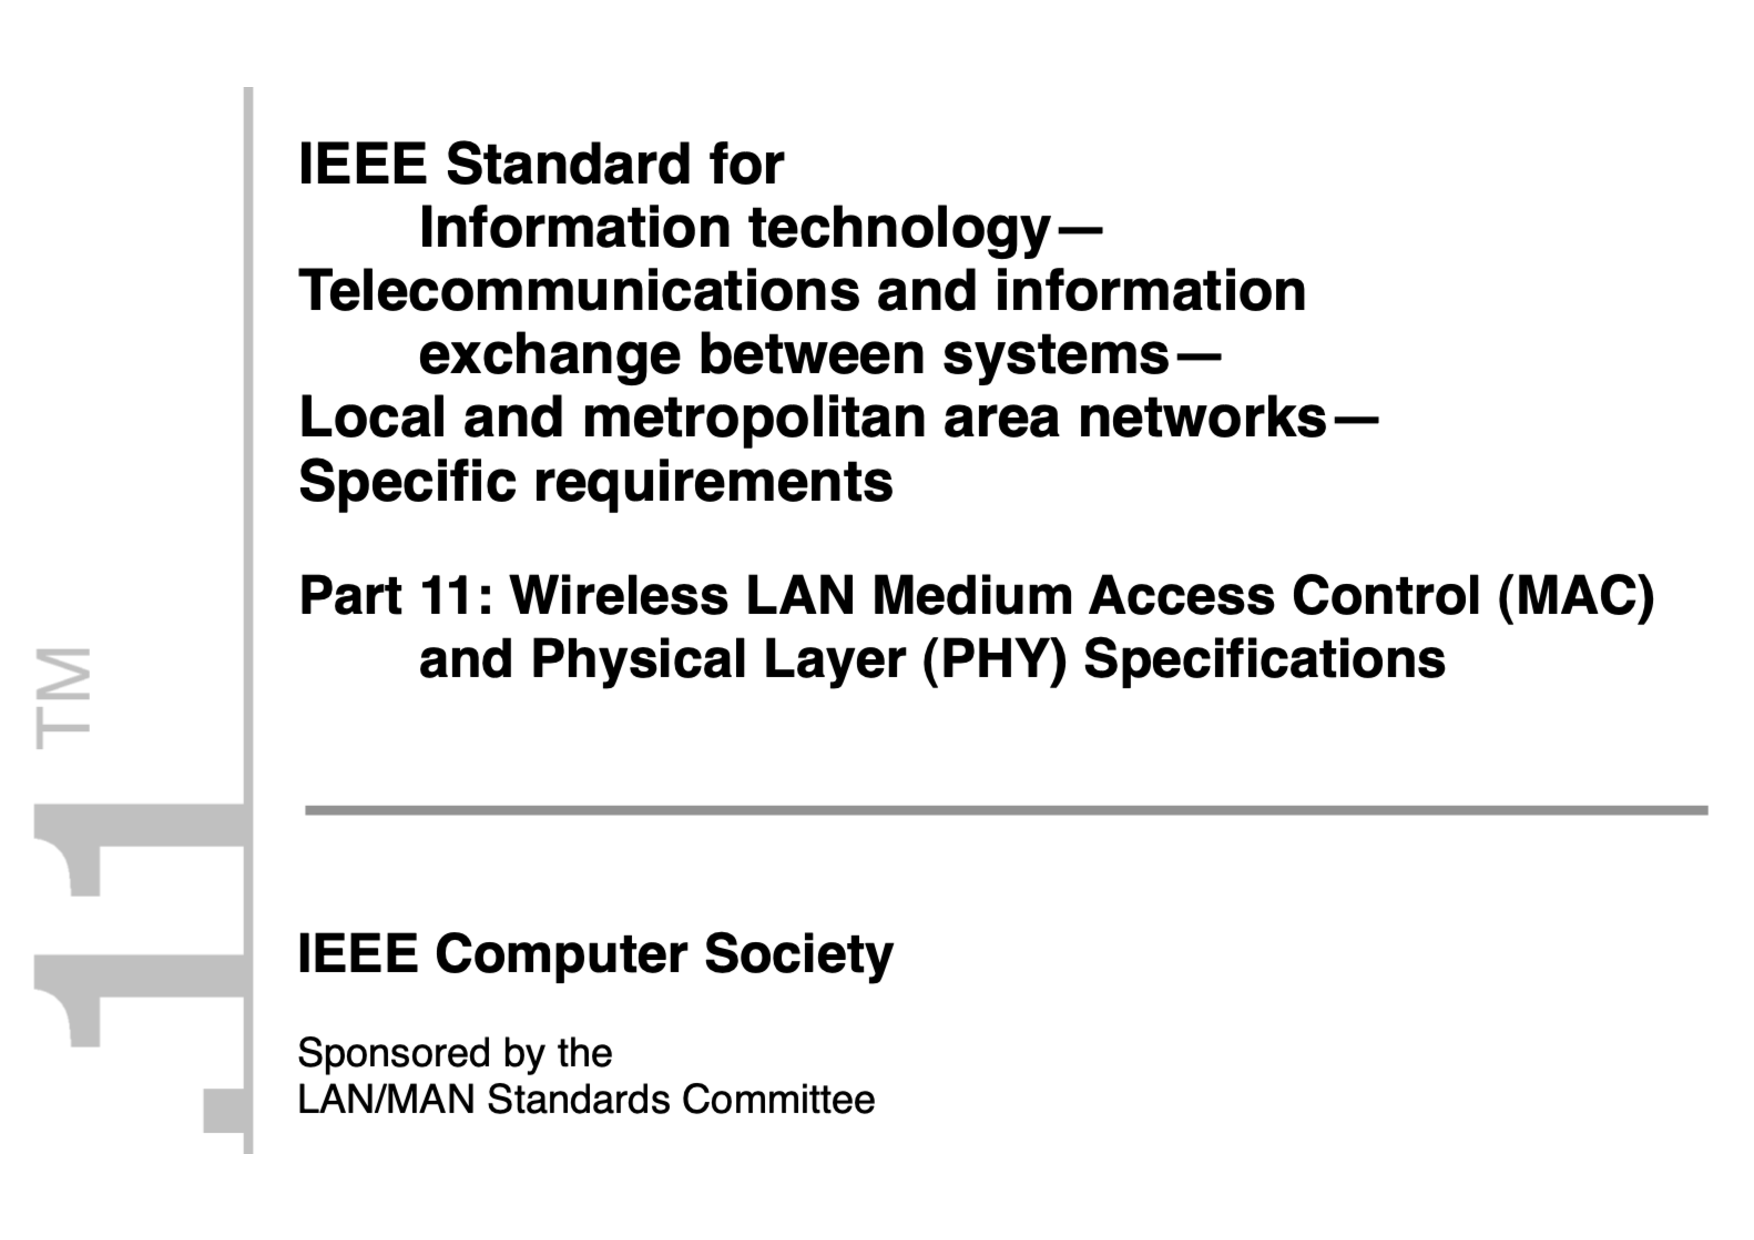
\includegraphics[width=0.9\textwidth]{./Figuras/Wifi1.pdf}
\end{frame}

\begin{frame}{Introducción}{Ejemplo}
  \centering 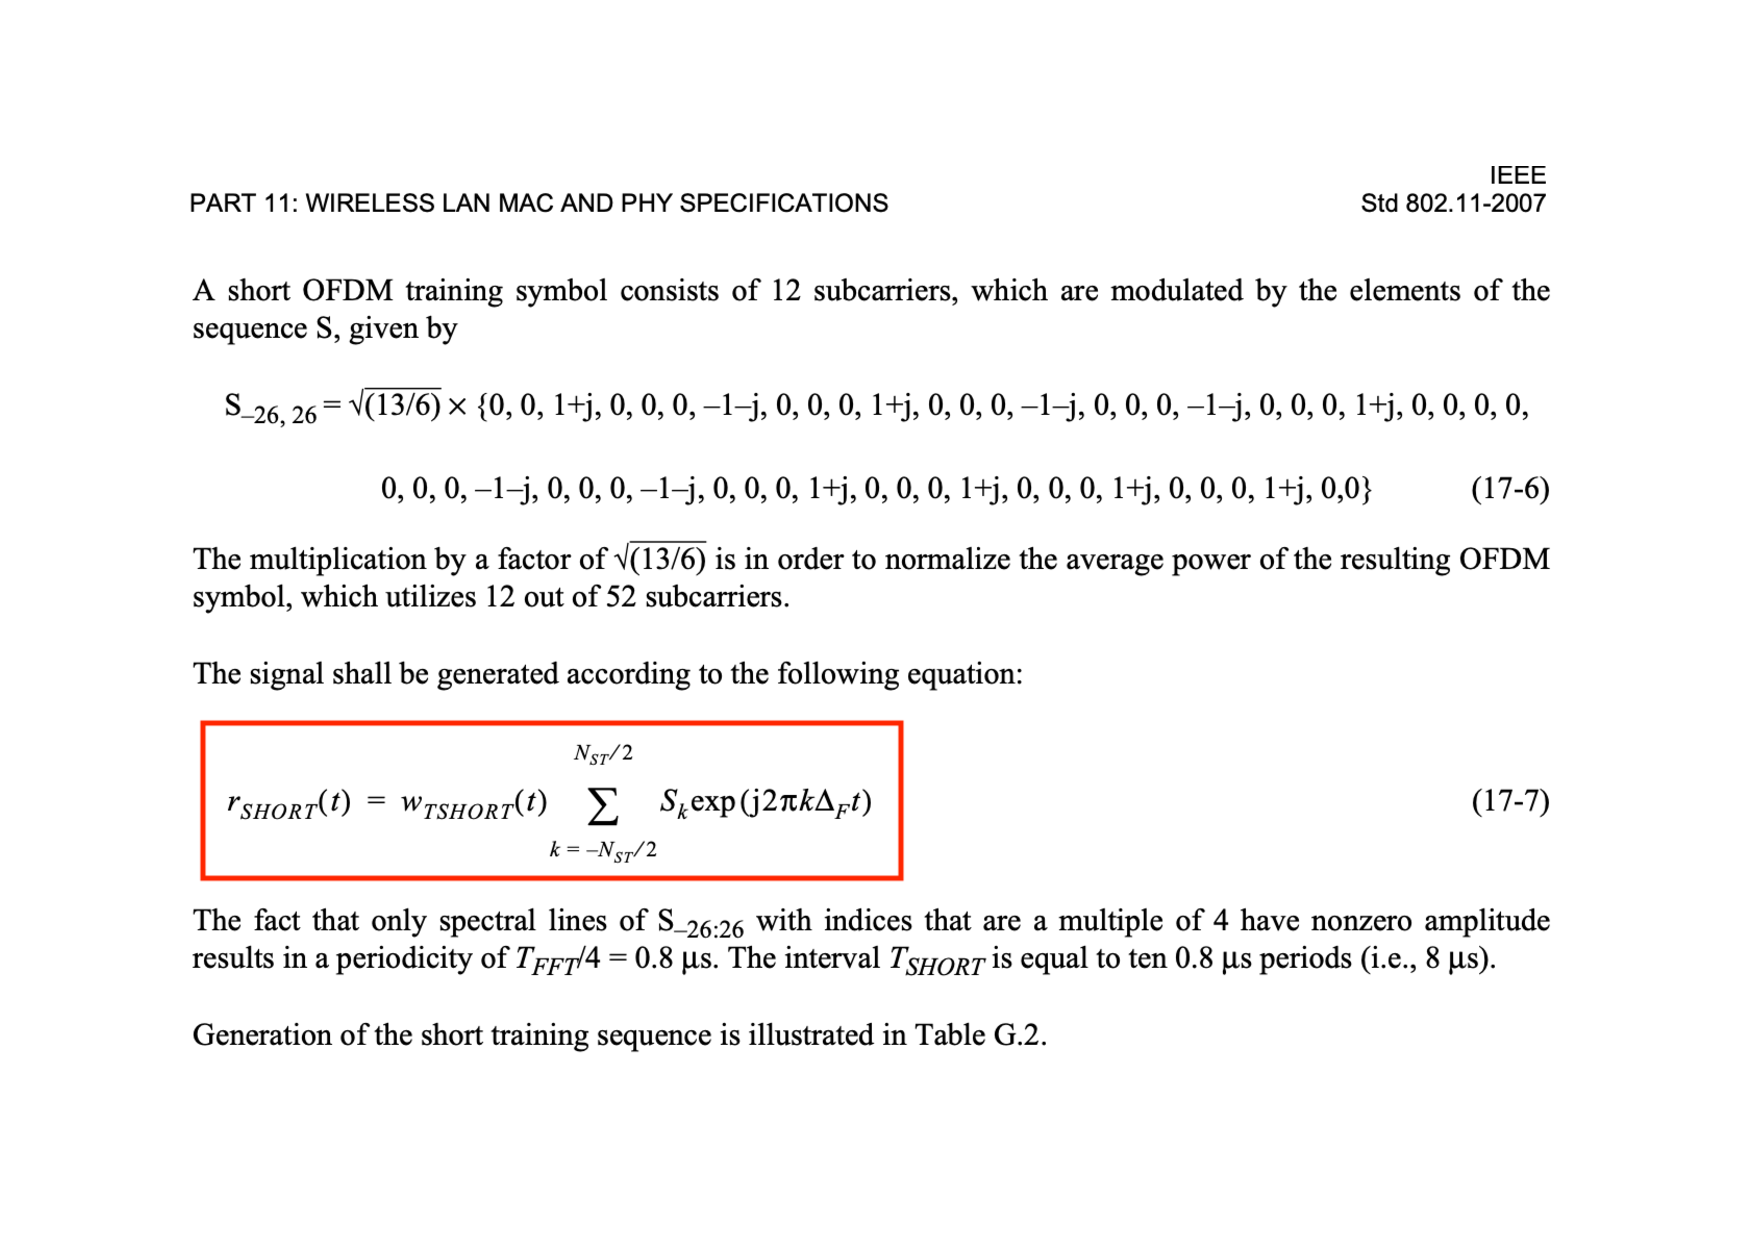
\includegraphics[width=0.9\textwidth]{./Figuras/Wifi2.pdf}
\end{frame}

\begin{frame}{Introducción}{Ejemplo}
  \centering 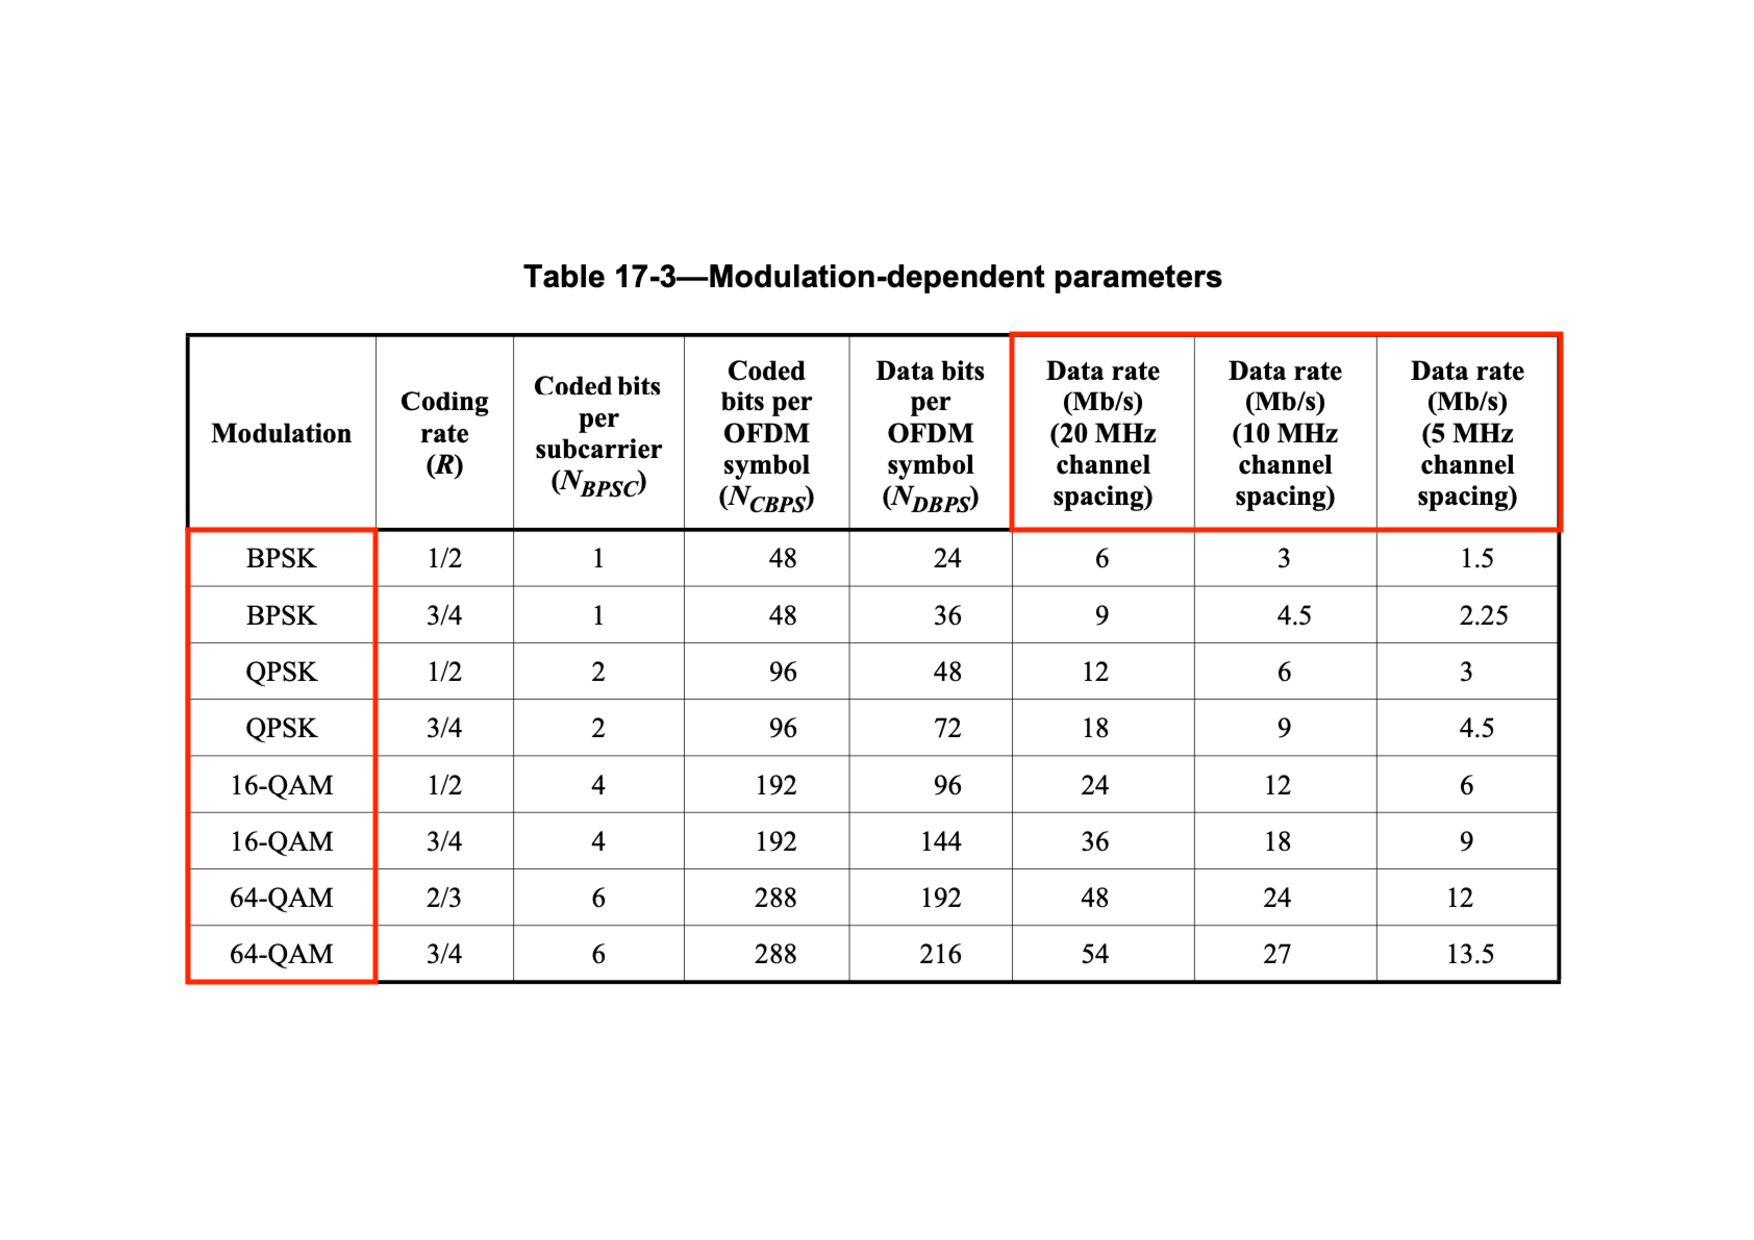
\includegraphics[width=0.9\textwidth]{./Figuras/Wifi3.pdf}
\end{frame}

\begin{frame}{Introducción}{Ejemplo}
  \centering 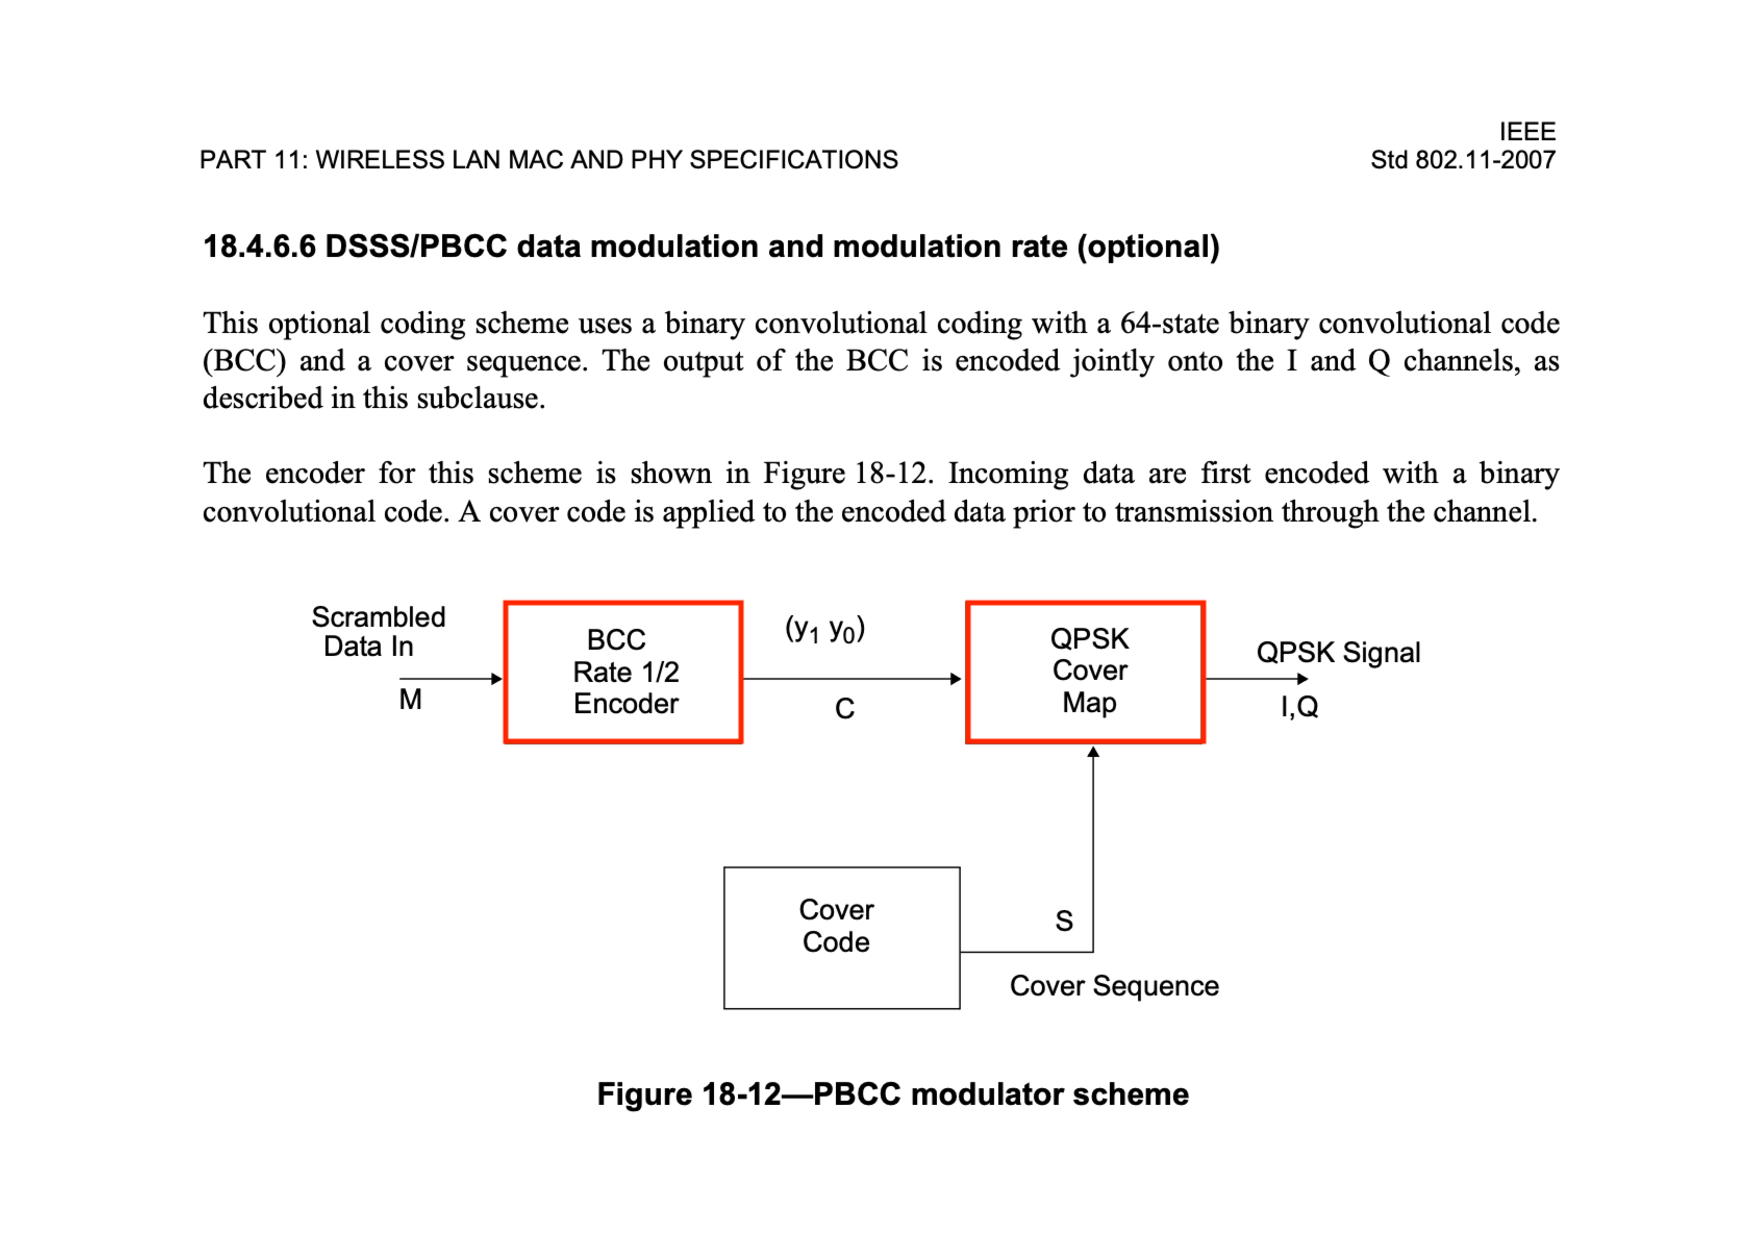
\includegraphics[width=0.9\textwidth]{./Figuras/Wifi4.pdf}
\end{frame}

\begin{frame}{Introducción}{Ejemplo}
  \centering 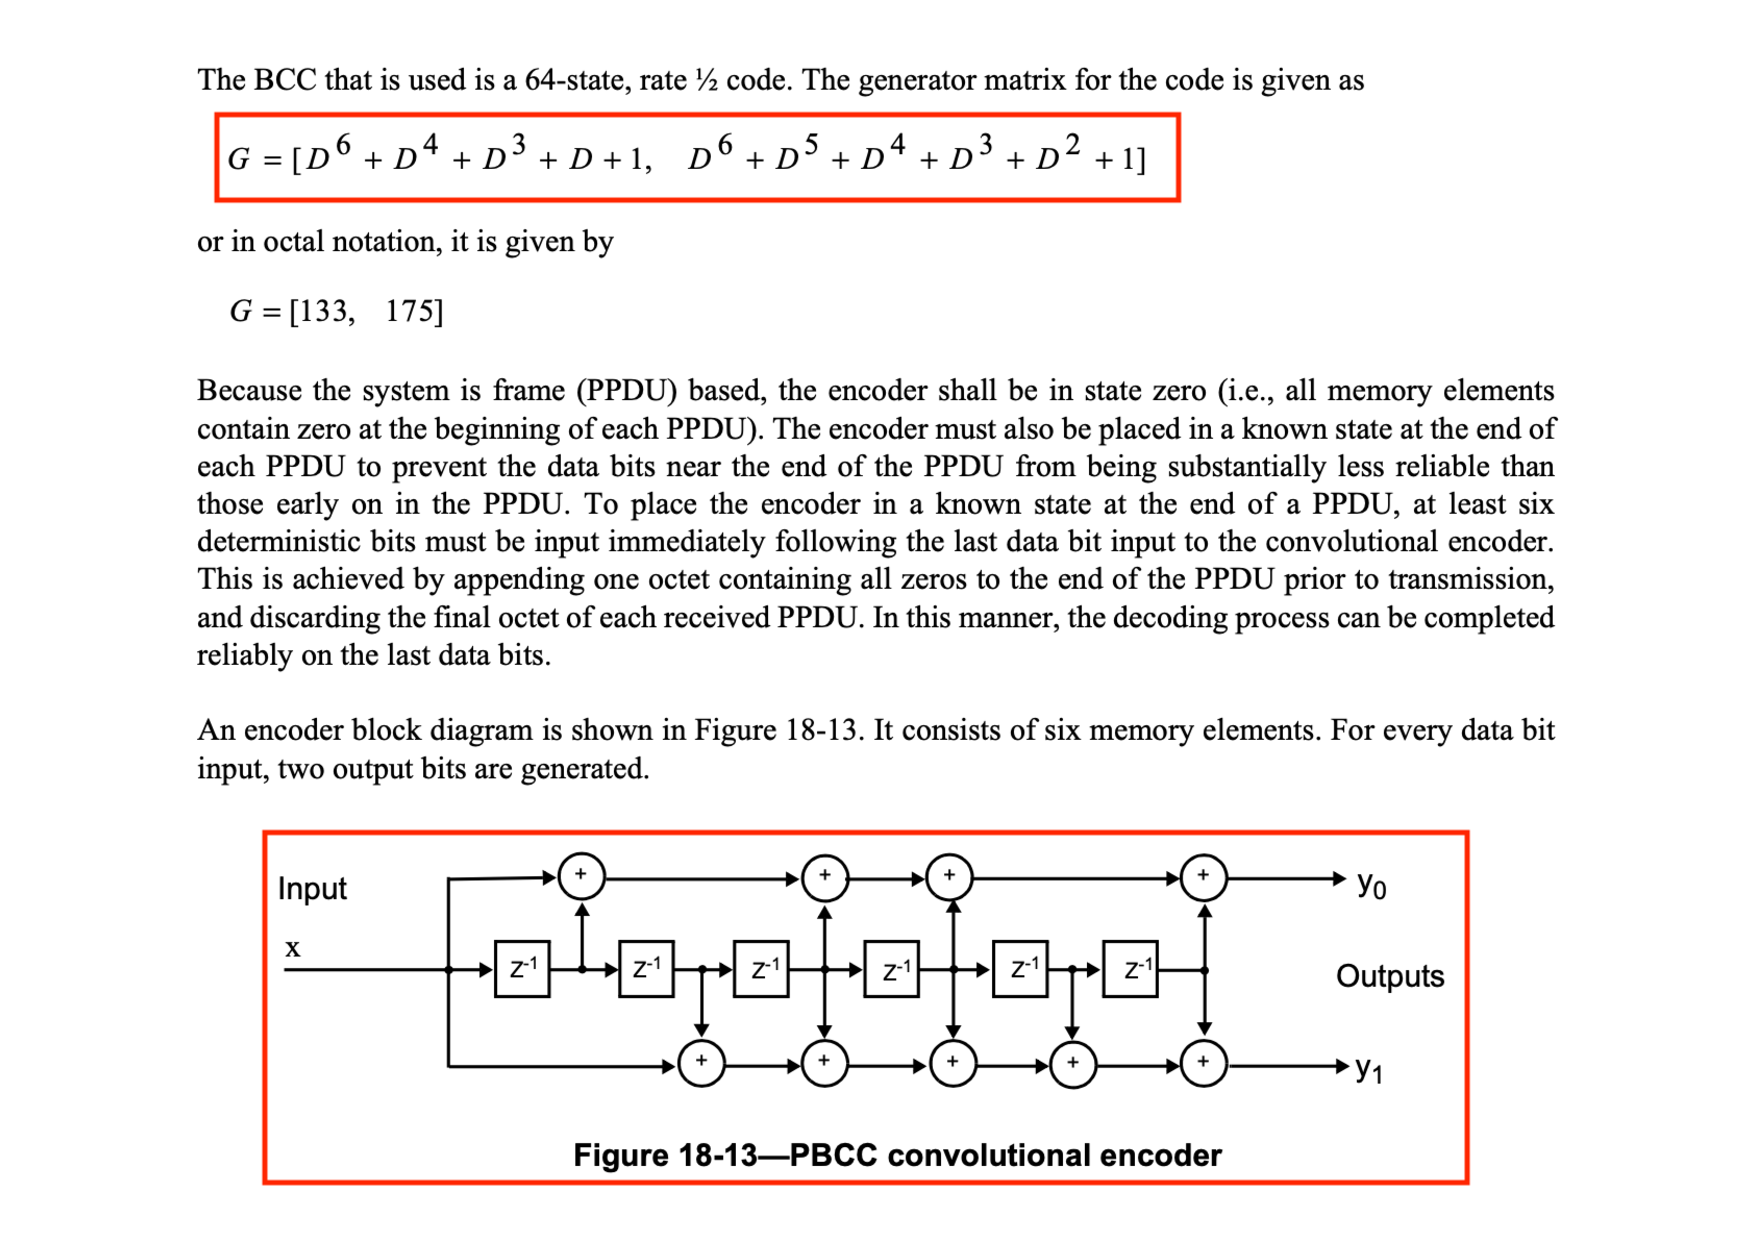
\includegraphics[width=0.9\textwidth]{./Figuras/Wifi5.pdf}
\end{frame}

\section{Teoría de la información}
\subsection{Medida de la información}
\begin{frame}{Teoría de la información}{Medida de la información}
    \begin{itemize}
		\item Se define la cantidad de información como:
		\begin{displaymath}
        I = -log_2(p_k)
    \end{displaymath}
      siendo $p_k$ la probabilidad de aparición de cada uno de los posibles símbolos de la fuente. 
    
    \item Se define la {\bf entropía} de una fuente como:
    \begin{displaymath}
      H = - \sum_{k=0}^{N-1}p_k \cdot  log_2(p_k)
    \end{displaymath}
    La entropía se mide en bits, e indica cuántos bits por símbolo como mínimo son necesarios para codificar la fuente.
	\end{itemize}
\end{frame}

\begin{frame}{Teoría de la información}{Codificación de fuente}
  \begin{itemize}
  \item {\bf Objetivo}: Reducir el número de bits necesarios para representar la salida de una fuente. 
  \item {\bf Teorema de Shannon}: El número mínimo de bits por símbolo nunca va a ser inferior al valor de la entropía de la fuente.
  \item Códigos fuente:
  \begin{itemize}
    \item Codificación Huffman: creada por David Huffmann.
    \item Codificación LZW: creada por Abraham Lempel, Jacob Ziv y Terry Welch. 
  \end{itemize}
\end{itemize}
\end{frame}

\subsection{Características de los códigos fuente}
\begin{frame}{Teoría de la información}{Características de los códigos fuente}
  \begin{itemize}
    \item {\bf Longitud media}: Se define como la longitud promedio de las palabras del código
    \begin{displaymath}
      \bar{L} = \sum_{i=1}^M p_i n_i	
    \end{displaymath}
    \item {\bf Tasa de compresión}: Se define como la relación frente a un código de longitud fija:
    \begin{displaymath}
      \Gamma = \frac{\lceil log_2 M \rceil}{\bar{L}}	
    \end{displaymath}
    \item {\bf Eficiencia}: Mide lo cerca que estamos del límite teórico de la entropía:
    \begin{displaymath}
      \eta = \frac{H(x)}{\bar{L}} \leq 1	
    \end{displaymath}
  \end{itemize}
\end{frame}


\section{Codificación Huffman}
\subsection{Introducción}

\begin{frame}{Codificación Huffman}{Introducción}
  \begin{itemize}
    \item Símbolos menos probables -> Se codifican con más bits
    \item Símbolos más probables -> Se codifican con menos bits
    \item El código se construye de forma iterativa en forma de árbol
  \end{itemize}
\end{frame}

\subsection{Ejemplo}
\begin{frame}{Codificación Huffman}{Ejemplo}
  \begin{itemize}
    \item Supongamos una fuente con nueve símbolos con las siguientes probabilidades:
    \begin{displaymath}
      \mathbf{p} = (0.2, 0.15, 0.13, 0.12, 0.1, 0.09, 0.08, 0.07, 0.06)
    \end{displaymath}
  \end{itemize}
\end{frame}

\begin{frame}{Codificación Huffman}{Ejemplo}
  \begin{itemize}
    \item Agrupo los dos símbolos menos probables en uno cuya probabilidad será la suma y reordeno:
  \end{itemize}
  \centering 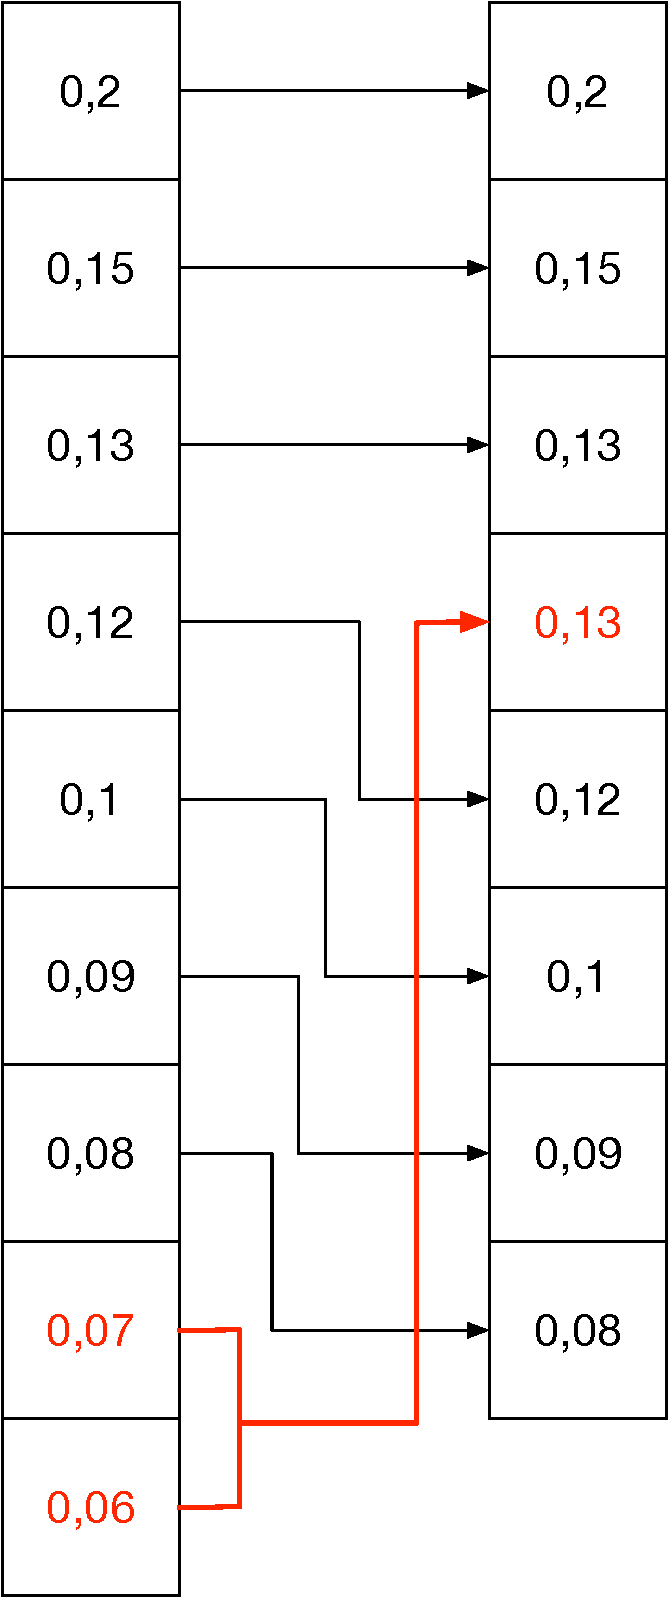
\includegraphics[height=5cm]{./Figuras/Huffman1.pdf}
\end{frame}

\begin{frame}{Codificación Huffman}{Ejemplo}
  \begin{itemize}
    \item Repito el proceso hasta que sólo queden dos símbolos:
  \end{itemize}
  \centering 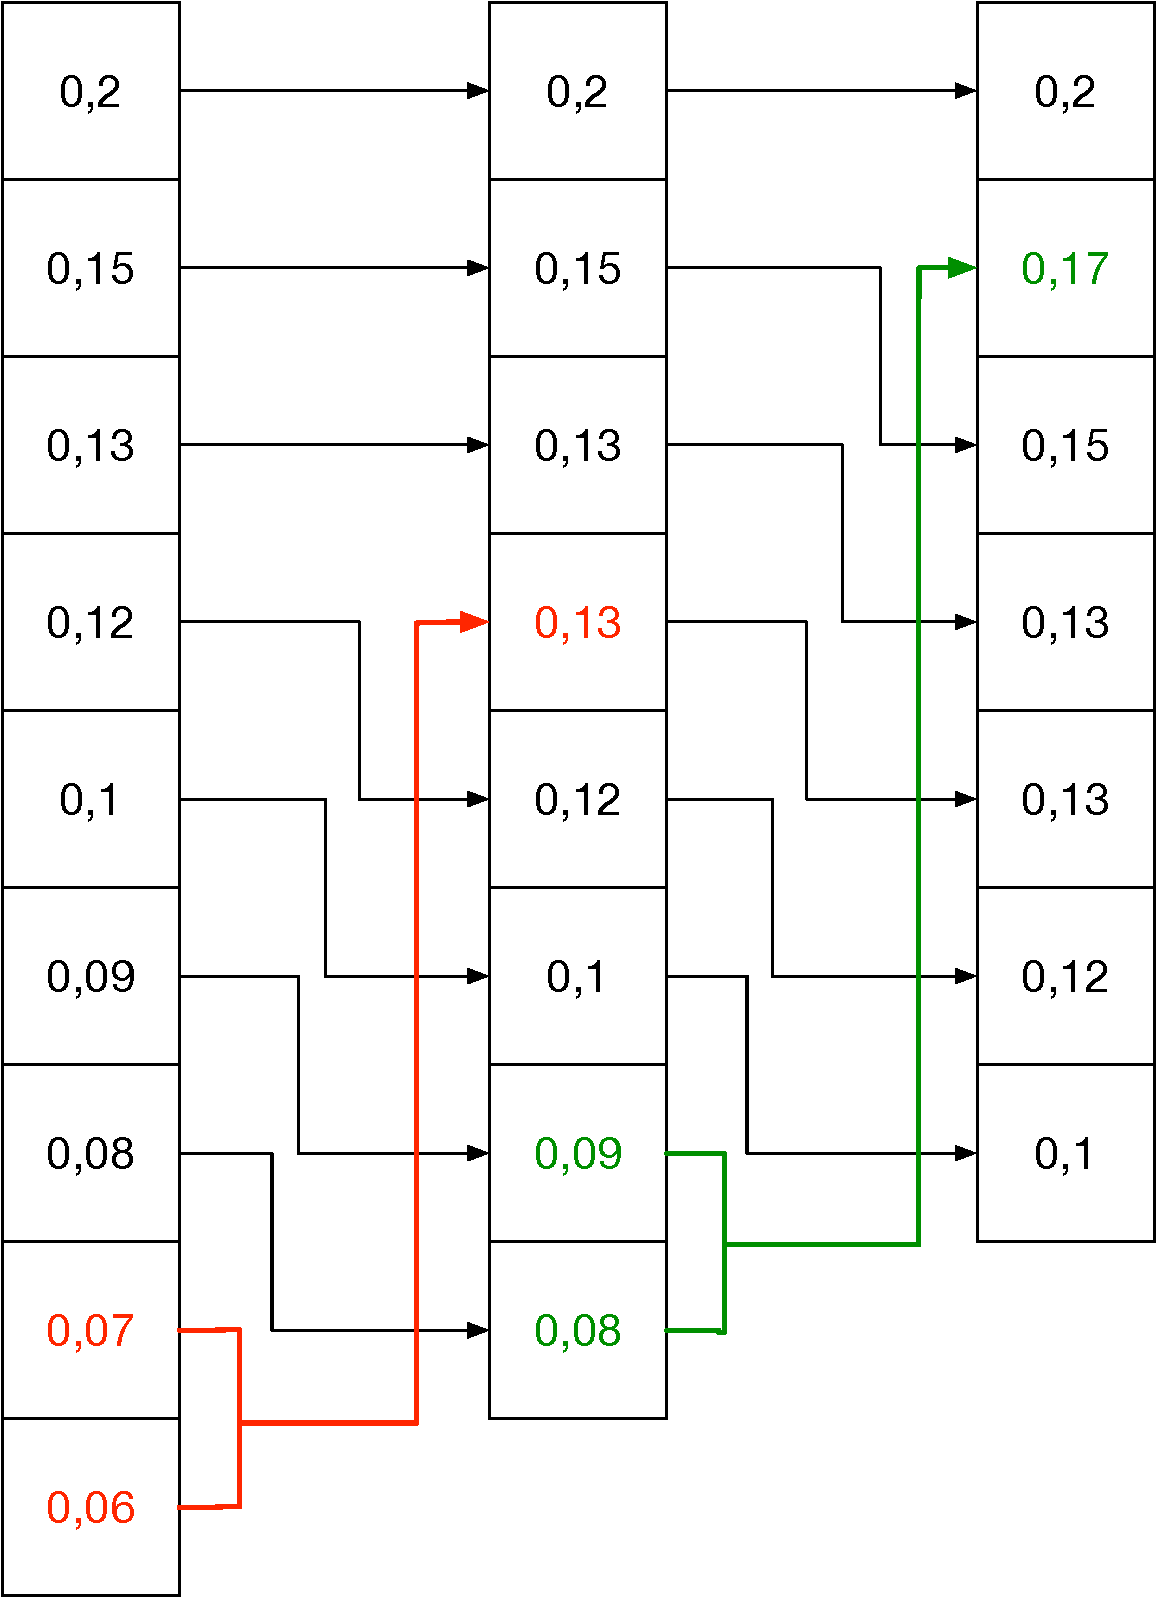
\includegraphics[height=5cm]{./Figuras/Huffman2.pdf}
\end{frame}

\begin{frame}{Codificación Huffman}{Ejemplo}
  \begin{itemize}
    \item Repito el proceso hasta que sólo queden dos símbolos:
  \end{itemize}
  \centering 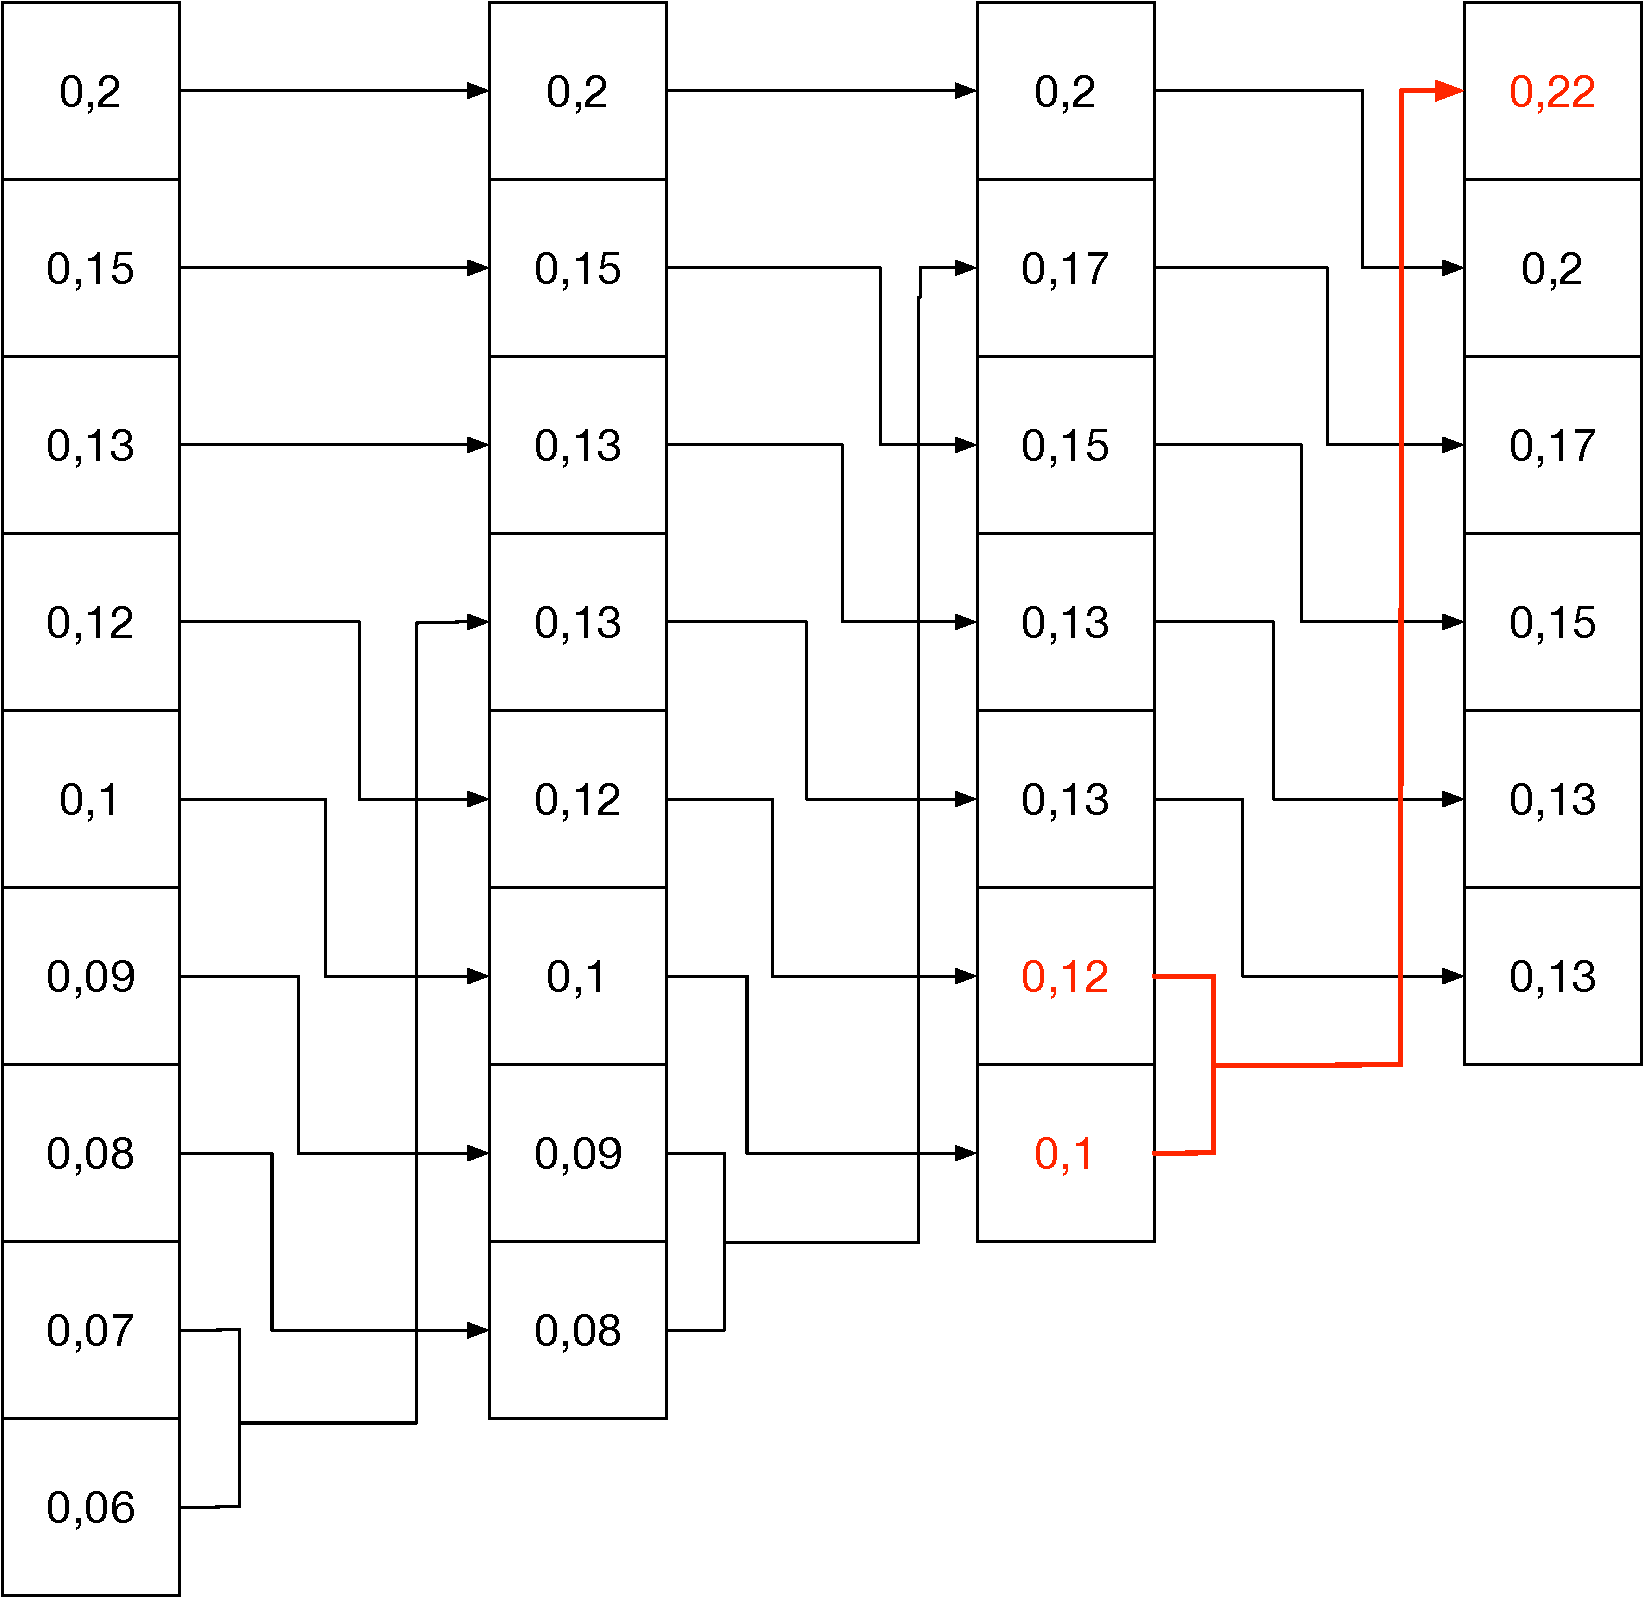
\includegraphics[height=5cm]{./Figuras/Huffman3.pdf}
\end{frame}

\begin{frame}{Codificación Huffman}{Ejemplo}
  \begin{itemize}
    \item Repito el proceso hasta que sólo queden dos símbolos:
  \end{itemize}
  \centering 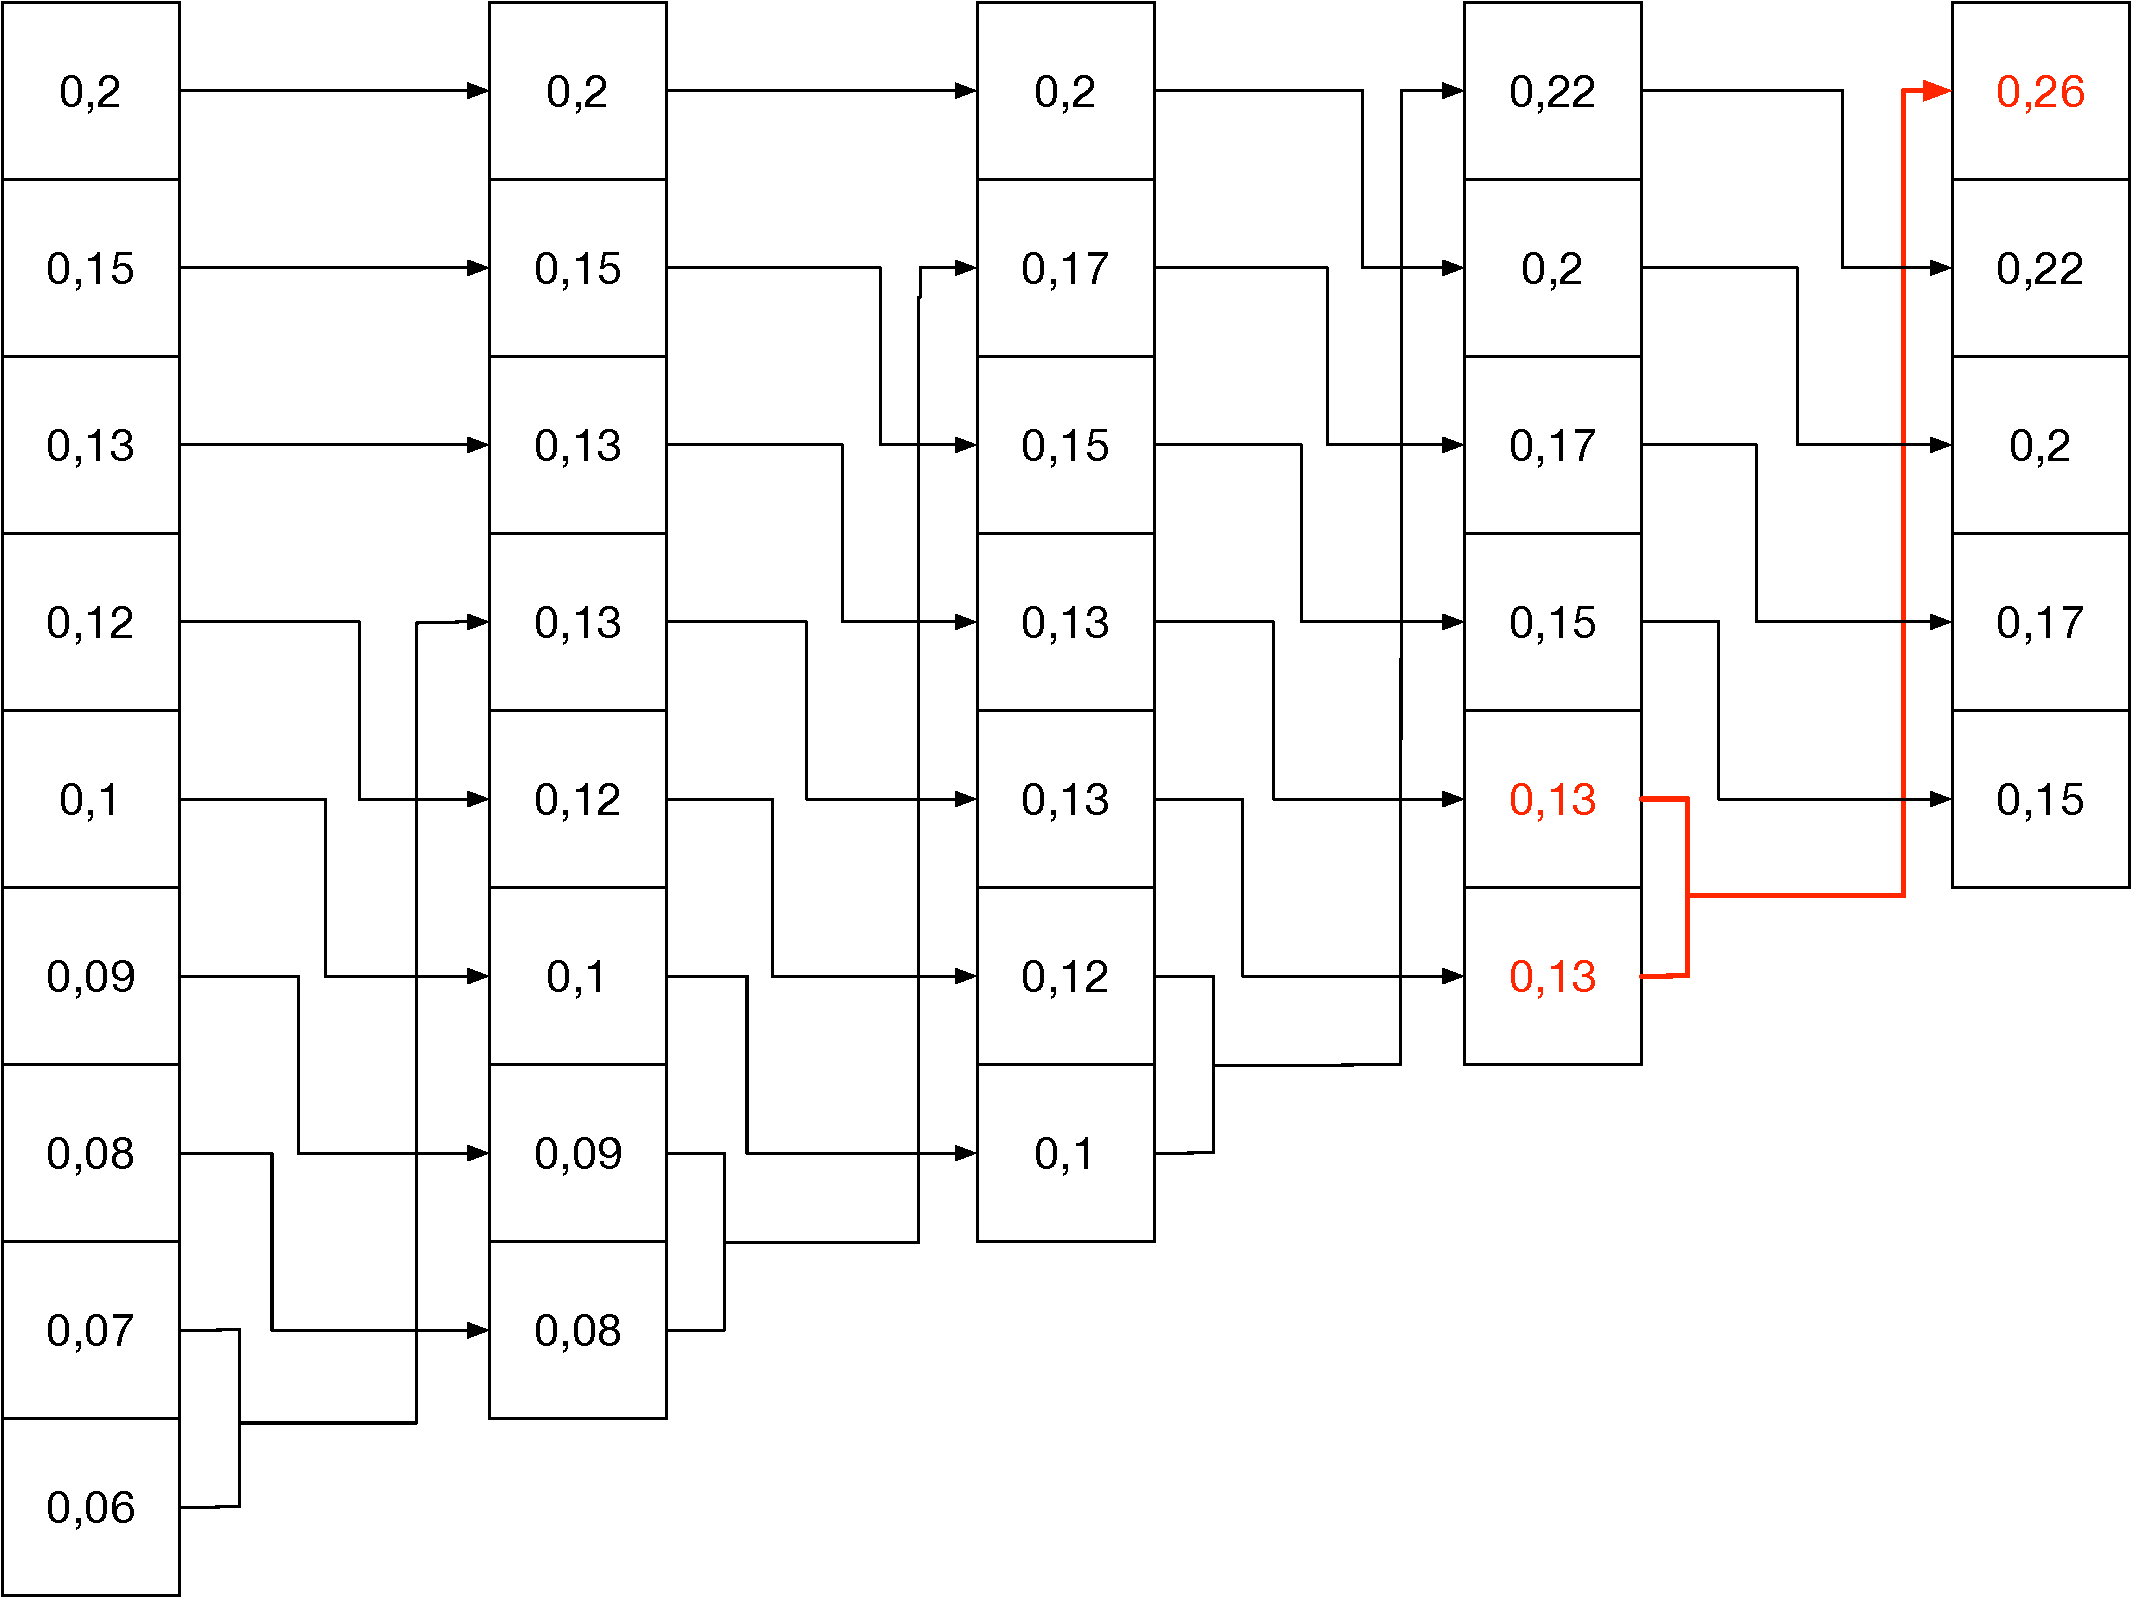
\includegraphics[height=5cm]{./Figuras/Huffman4.pdf}
\end{frame}

\begin{frame}{Codificación Huffman}{Ejemplo}
  \begin{itemize}
    \item Repito el proceso hasta que sólo queden dos símbolos:
  \end{itemize}
  \centering 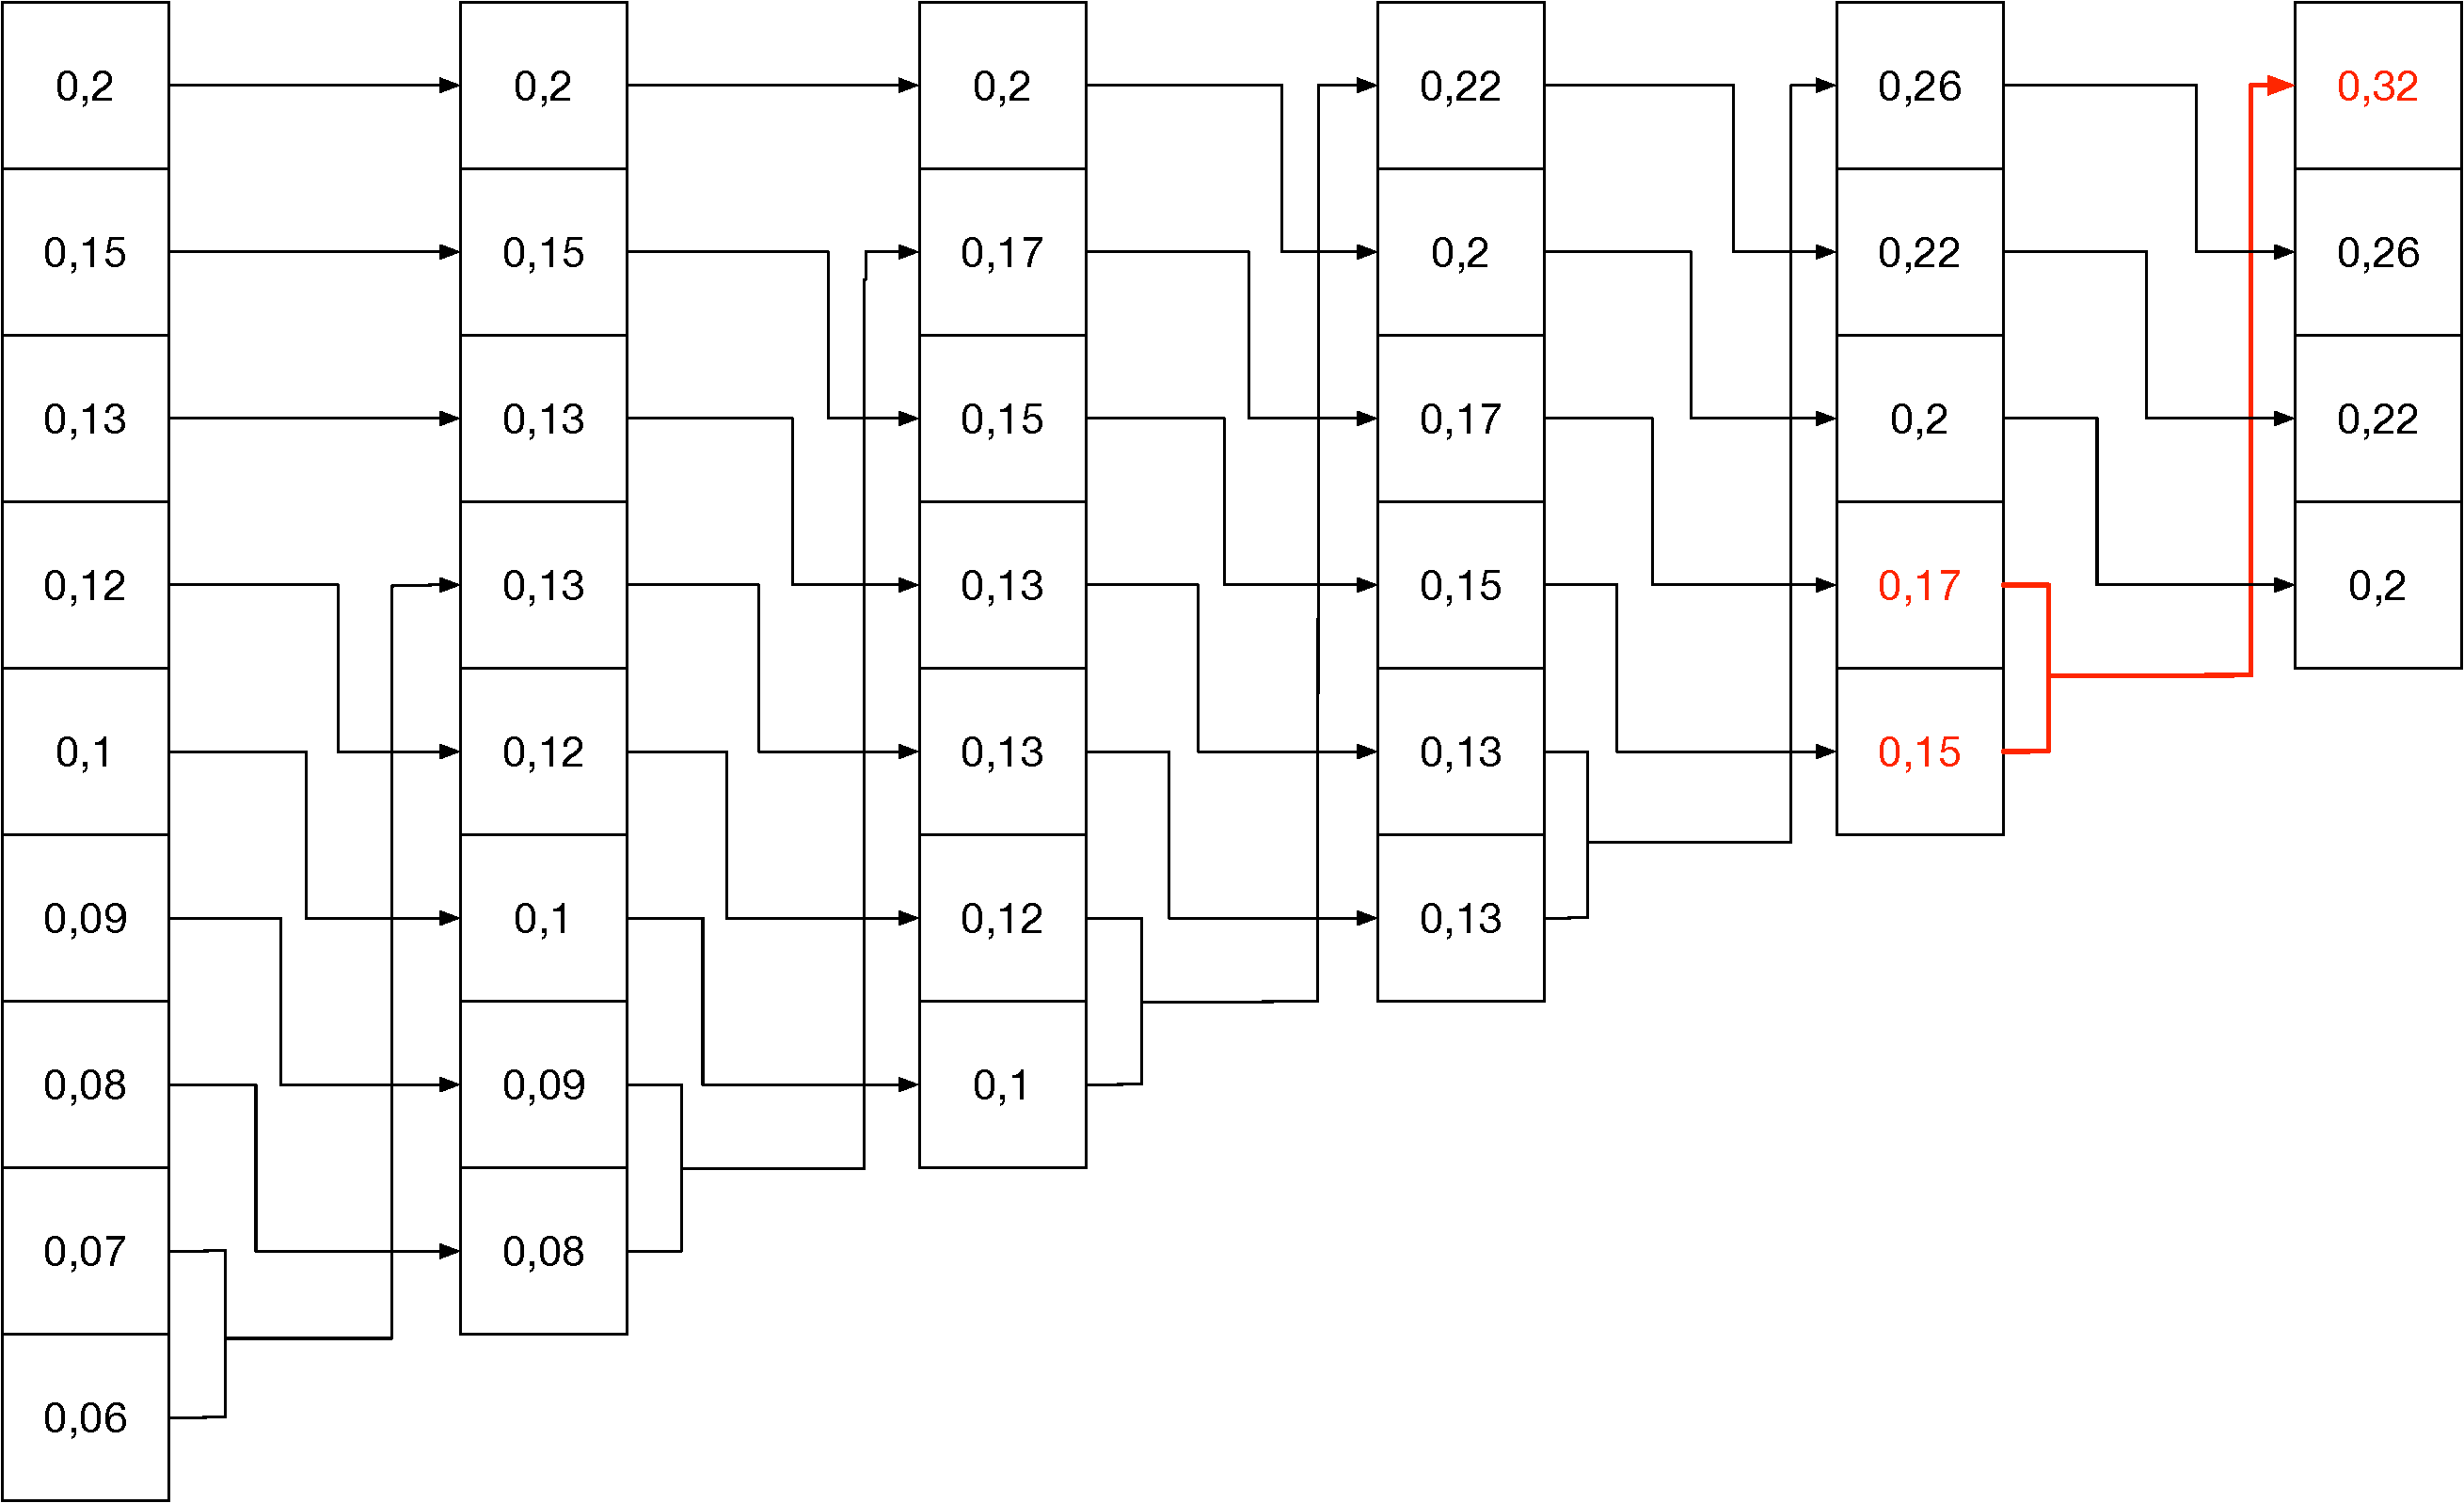
\includegraphics[height=5cm]{./Figuras/Huffman5.pdf}
\end{frame}

\begin{frame}{Codificación Huffman}{Ejemplo}
  \begin{itemize}
    \item Repito el proceso hasta que sólo queden dos símbolos:
  \end{itemize}
  \centering 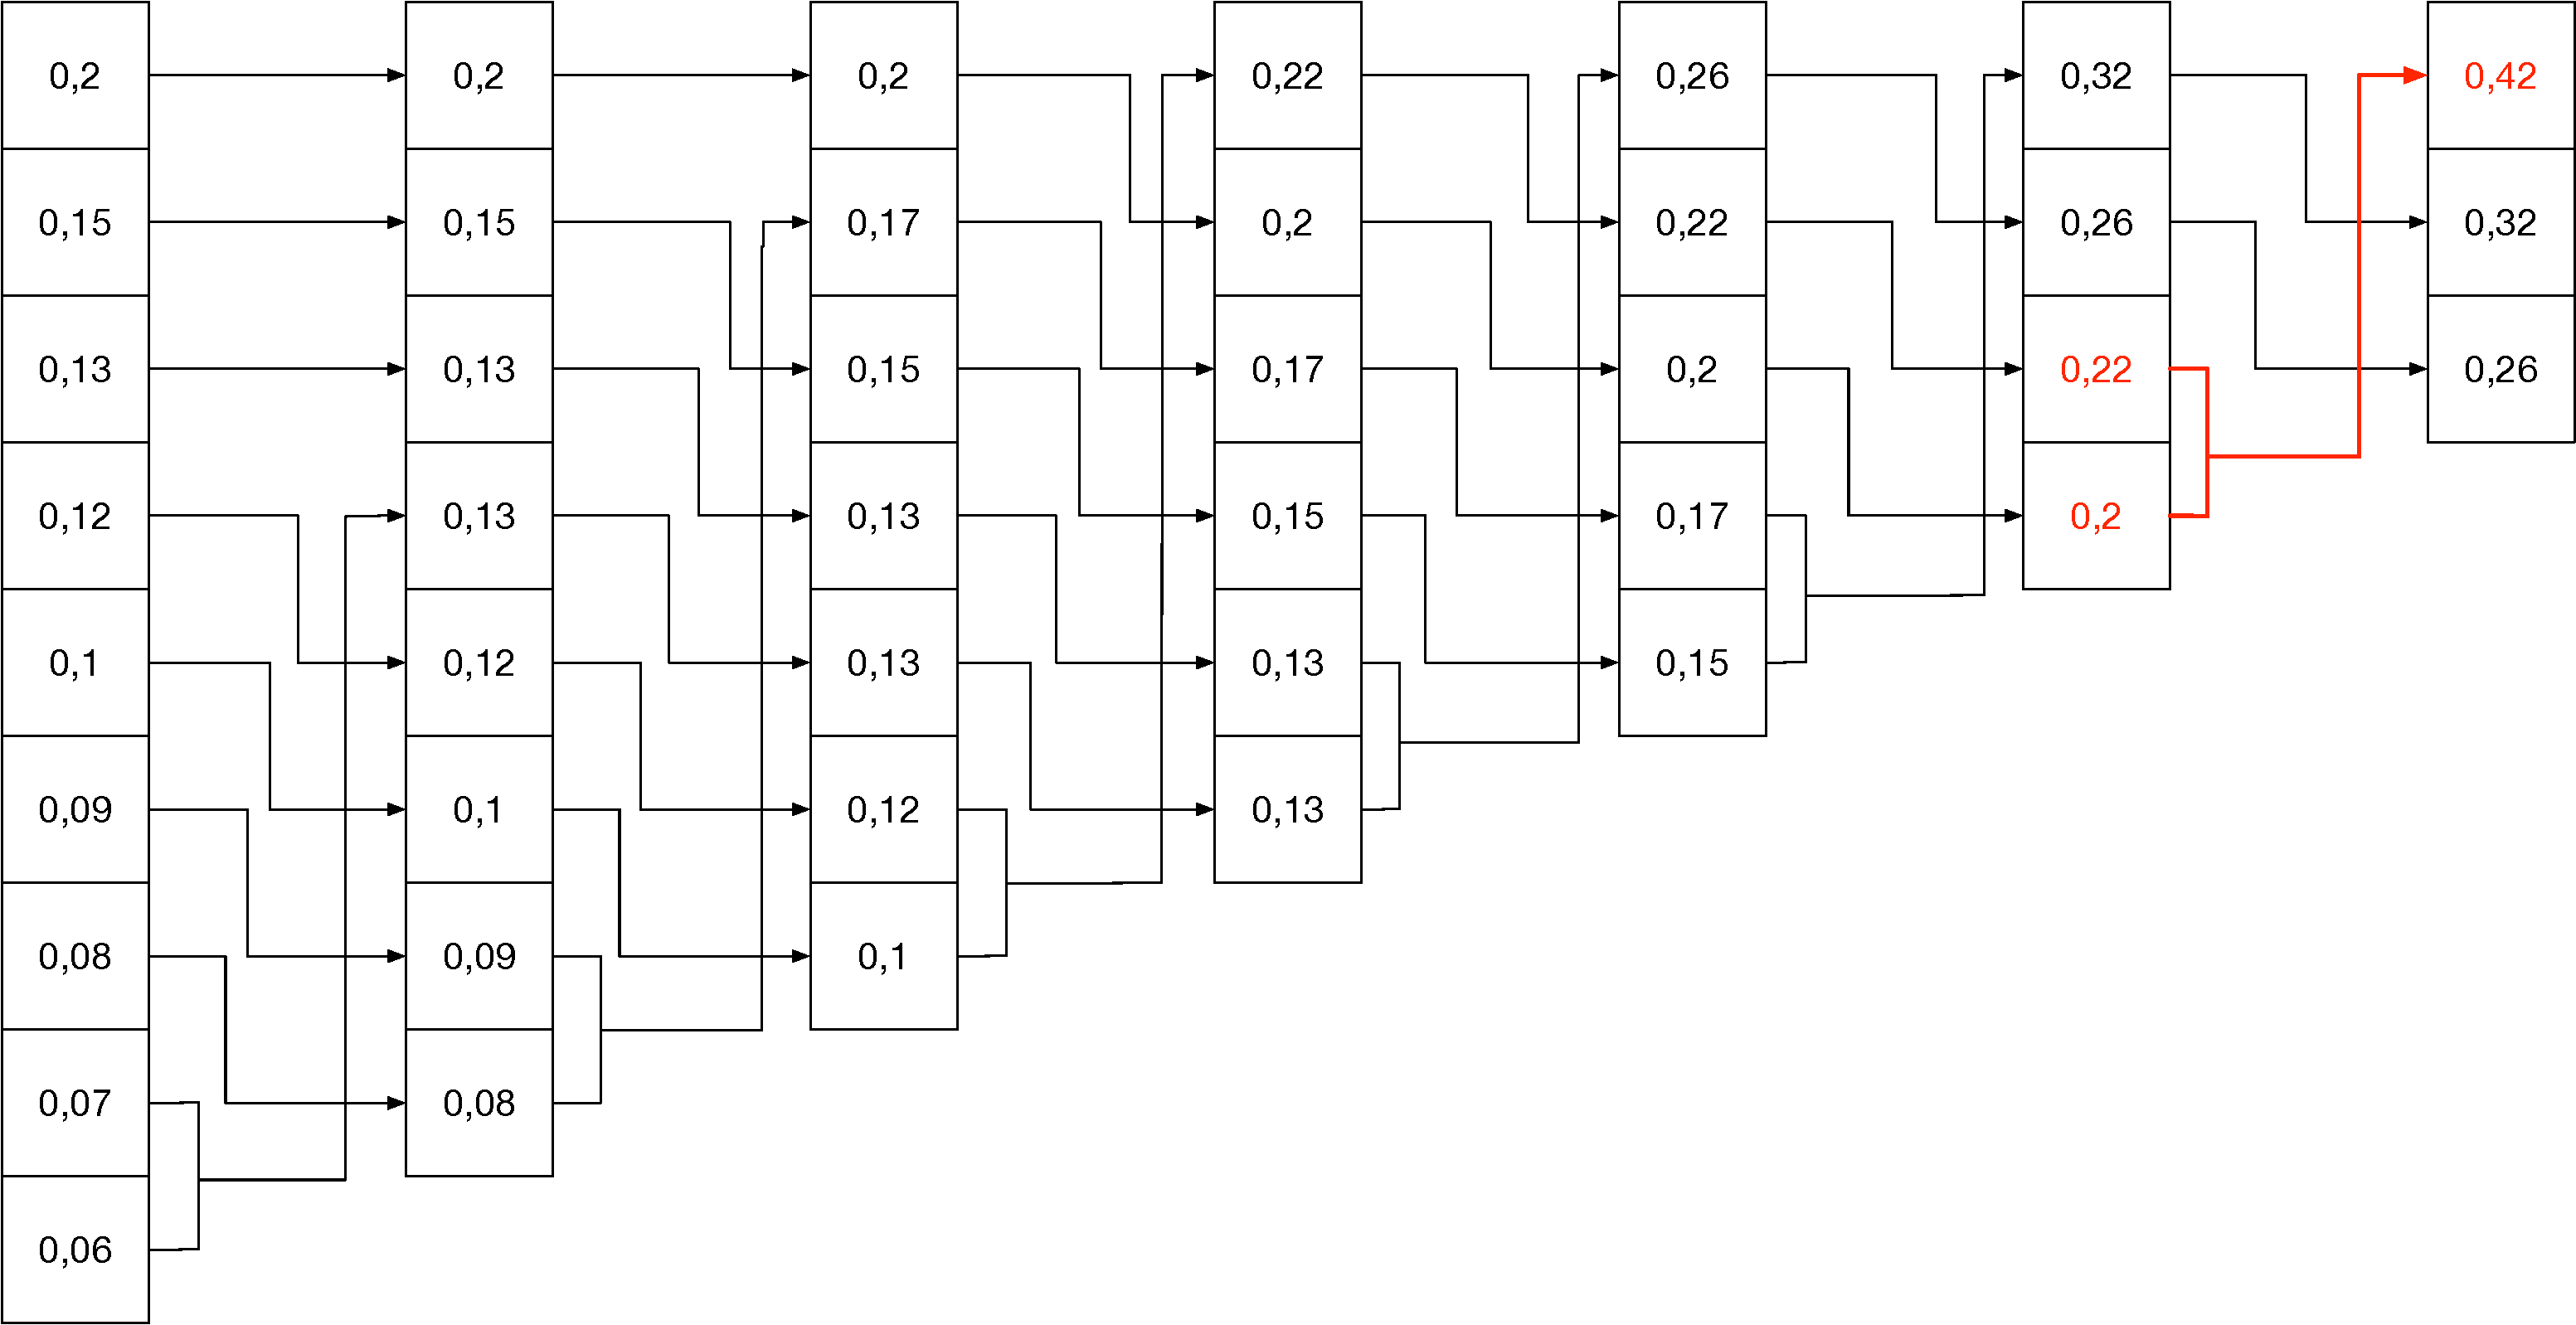
\includegraphics[height=5cm]{./Figuras/Huffman6.pdf}
\end{frame}

\begin{frame}{Codificación Huffman}{Ejemplo}
  \begin{itemize}
    \item Repito el proceso hasta que sólo queden dos símbolos:
  \end{itemize}
  \centering 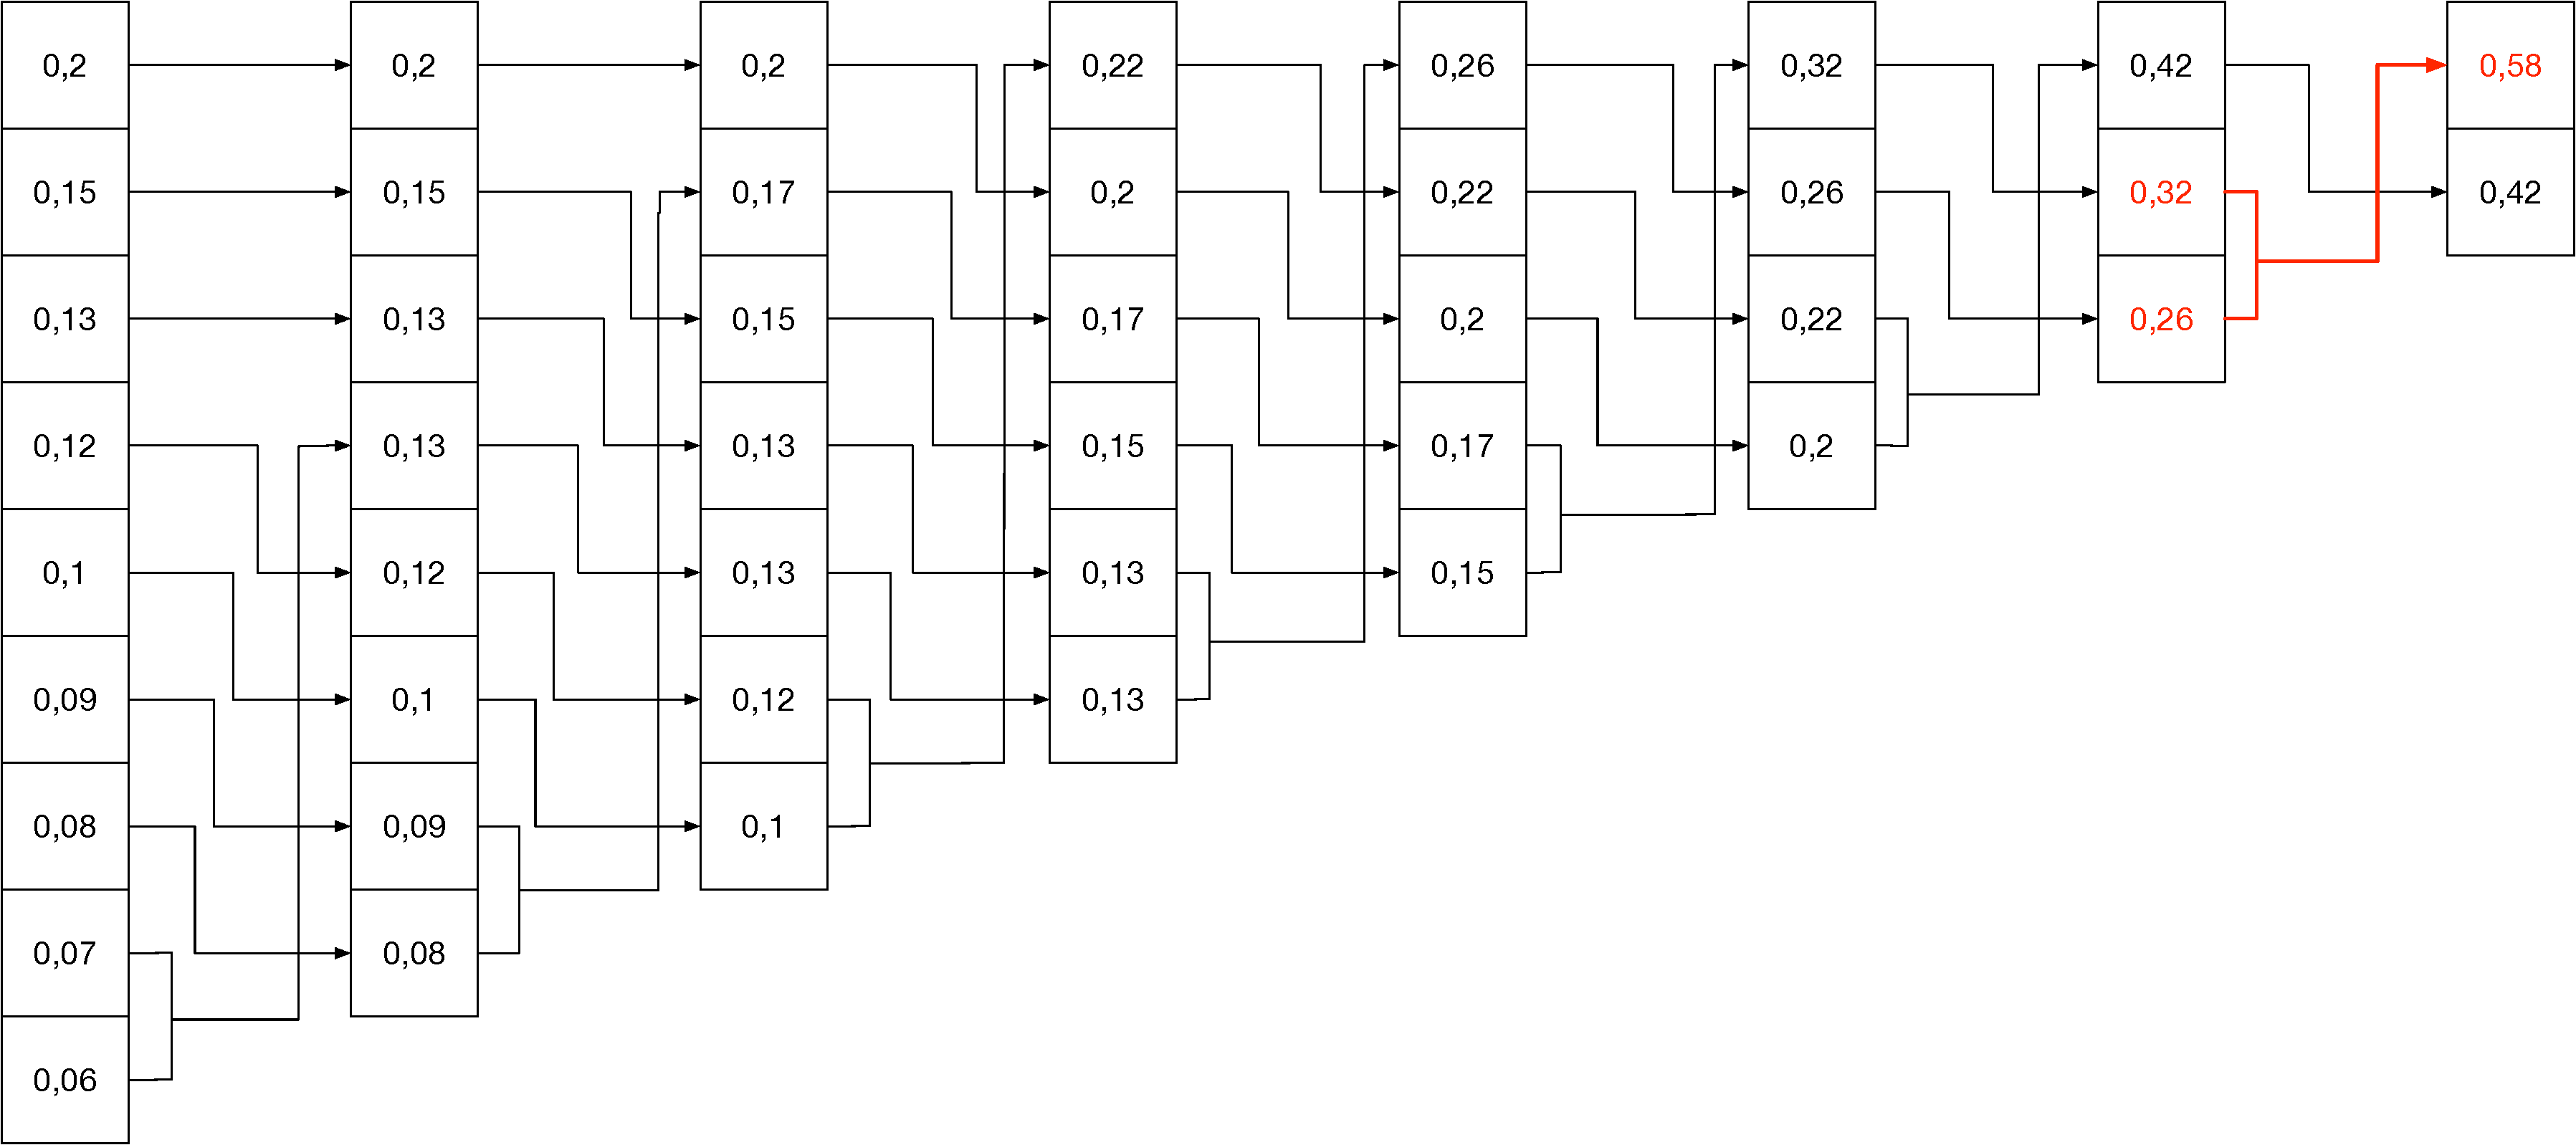
\includegraphics[height=5cm]{./Figuras/Huffman7.pdf}
\end{frame}

\begin{frame}{Codificación Huffman}{Ejemplo}
  \begin{itemize}
    \item Asigno '0' a un símbolo y '1' al otro:
  \end{itemize}
  \centering 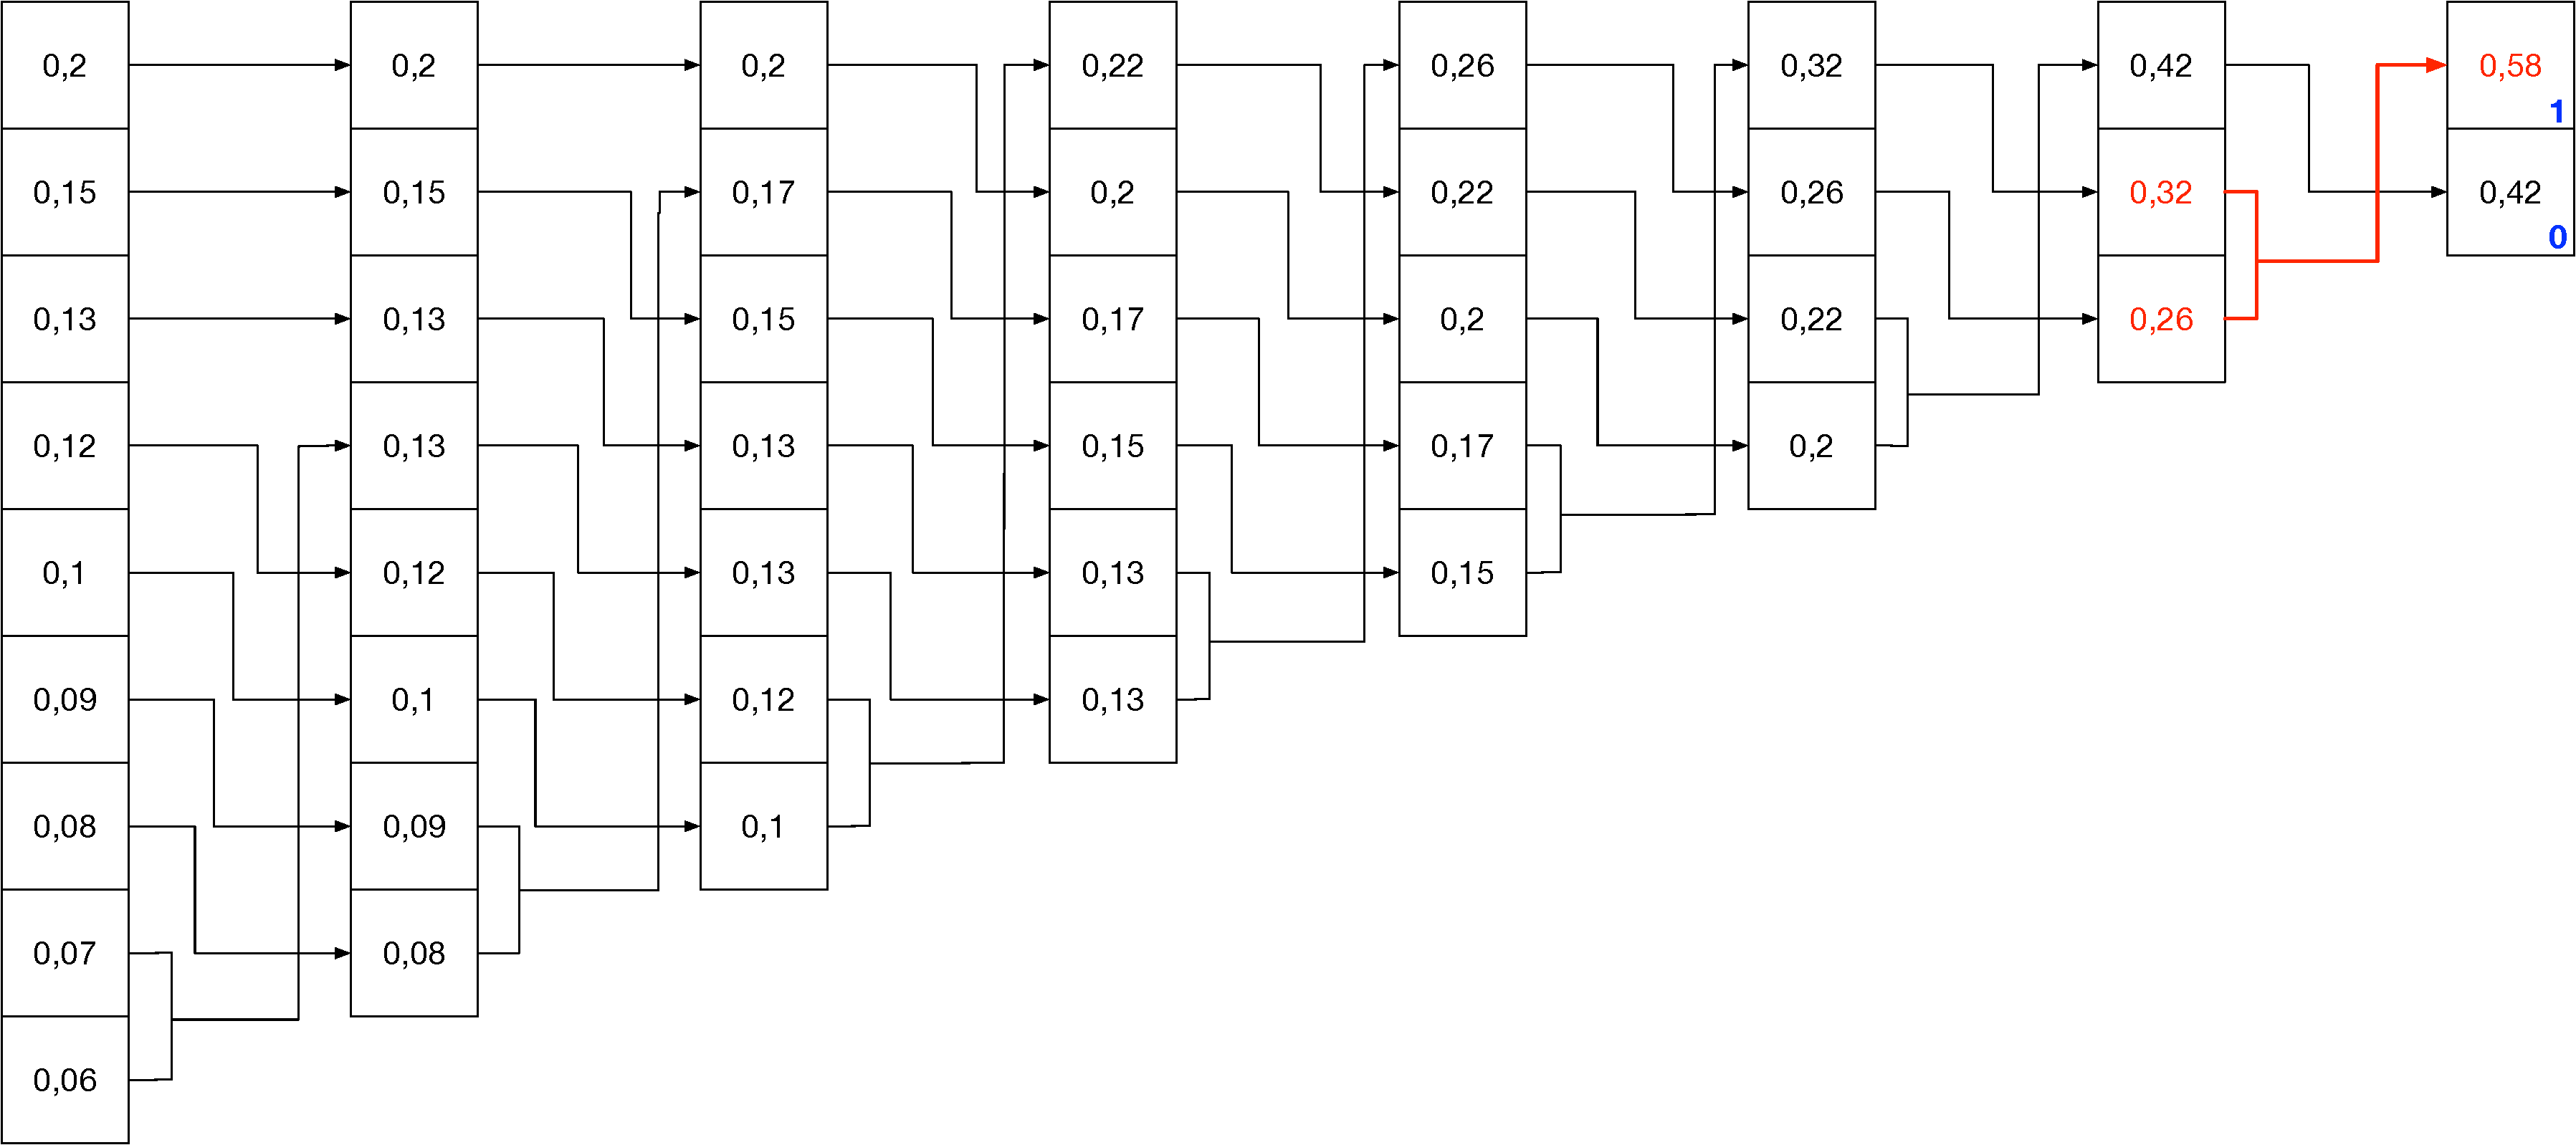
\includegraphics[height=5cm]{./Figuras/Huffman8.pdf}
\end{frame}

\begin{frame}{Codificación Huffman}{Ejemplo}
  \begin{itemize}
    \item Voy hacia atrás, añadiendo '0' ó '1' según corresponda:
  \end{itemize}
  \centering 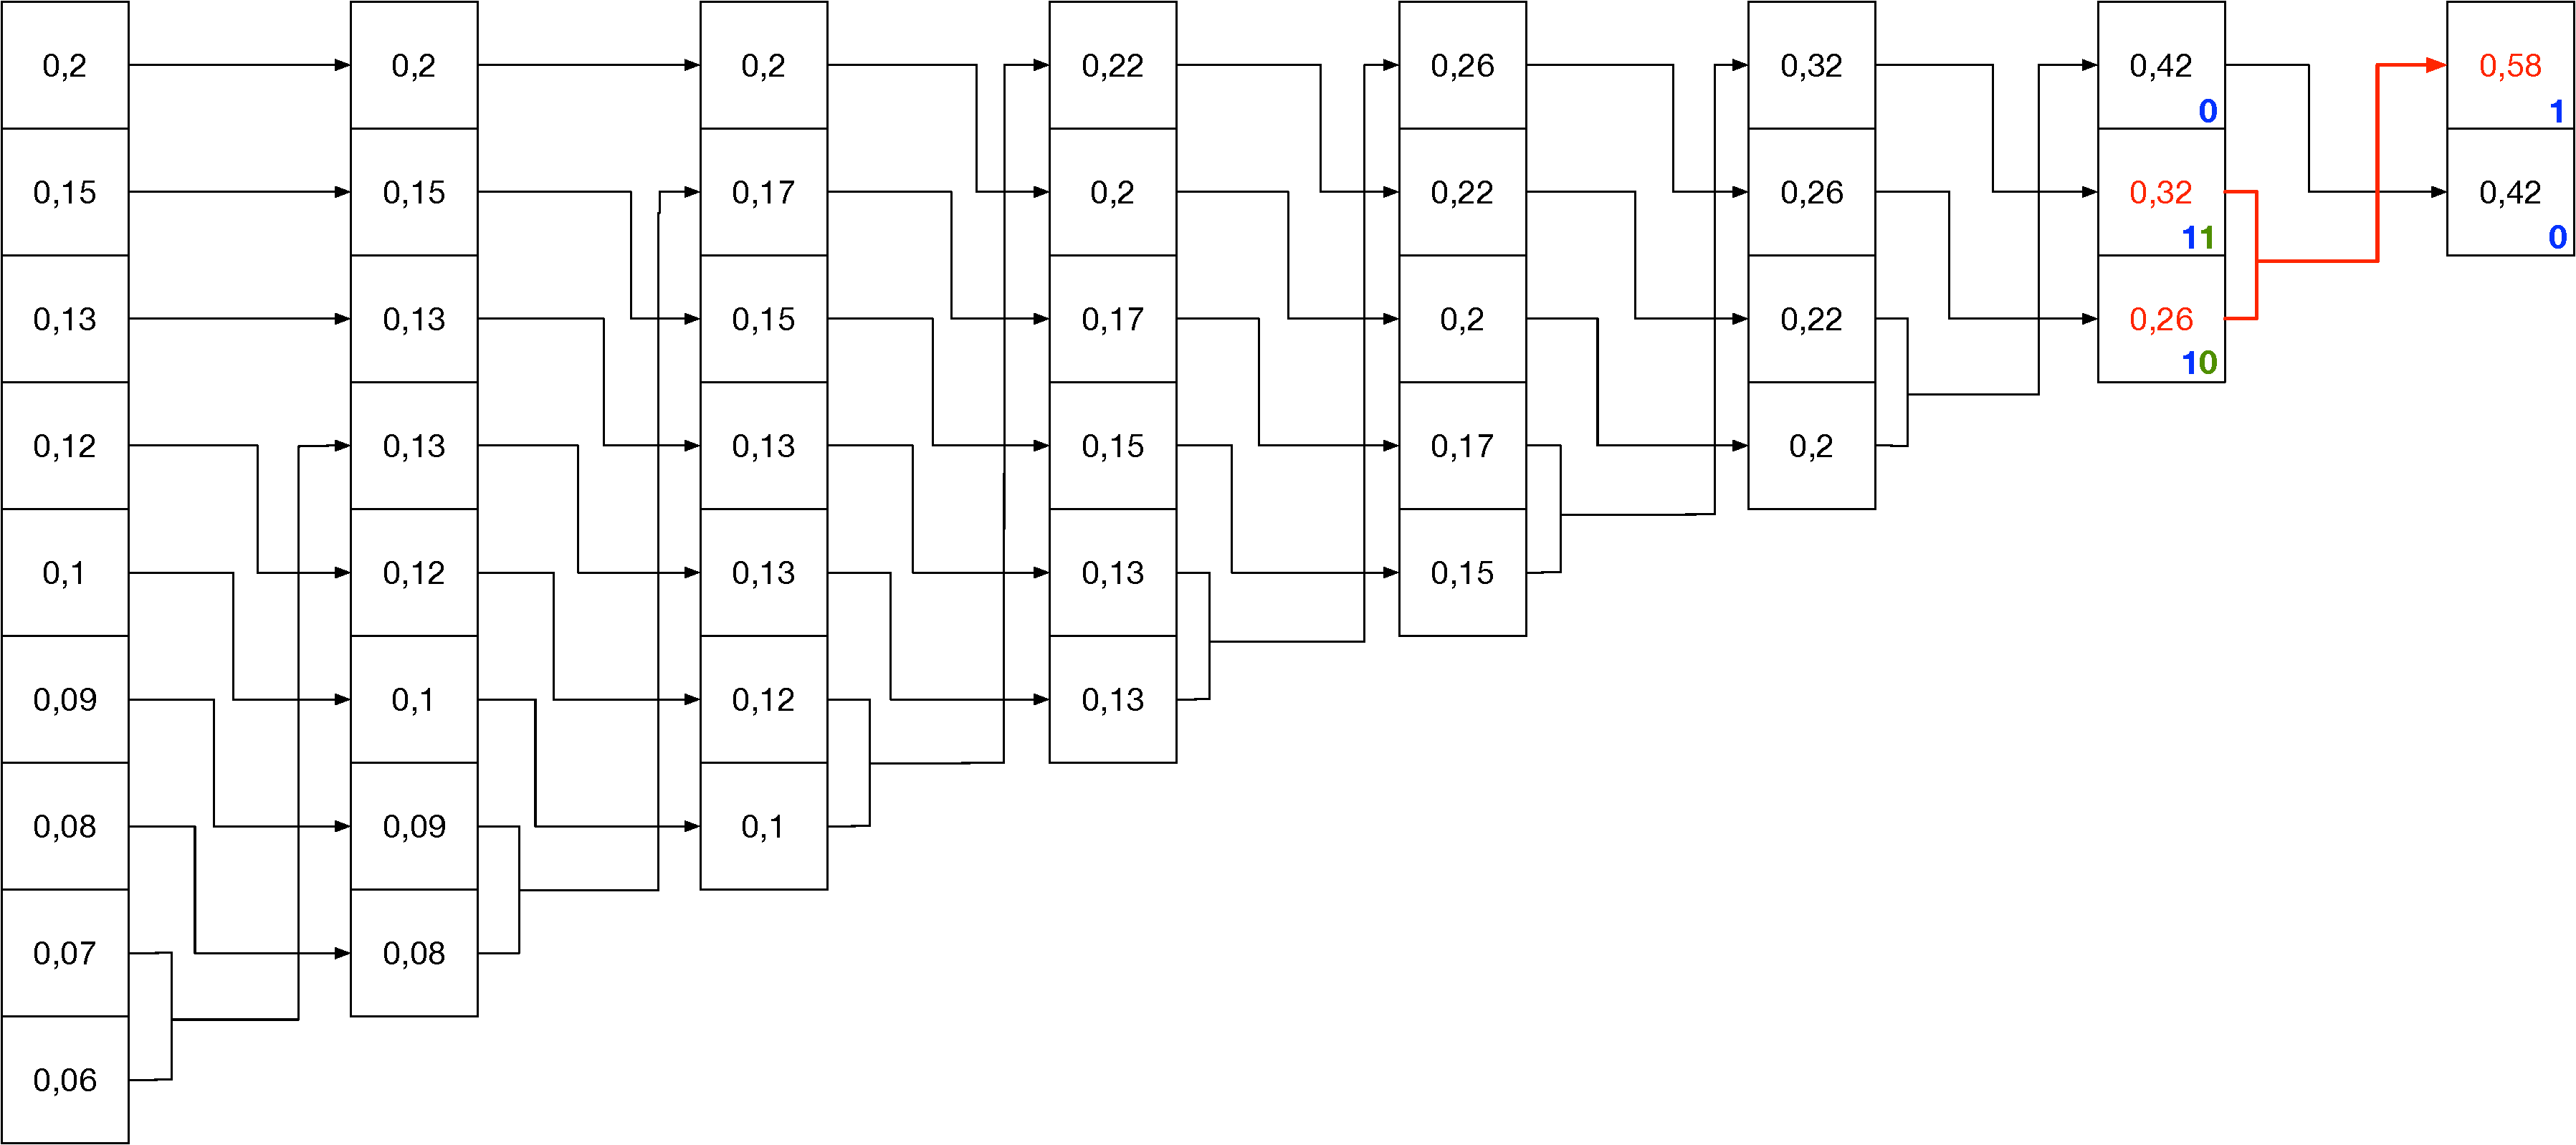
\includegraphics[height=5cm]{./Figuras/Huffman9.pdf}
\end{frame}

\begin{frame}{Codificación Huffman}{Ejemplo}
  \begin{itemize}
    \item Completo el proceso:
  \end{itemize}
  \centering 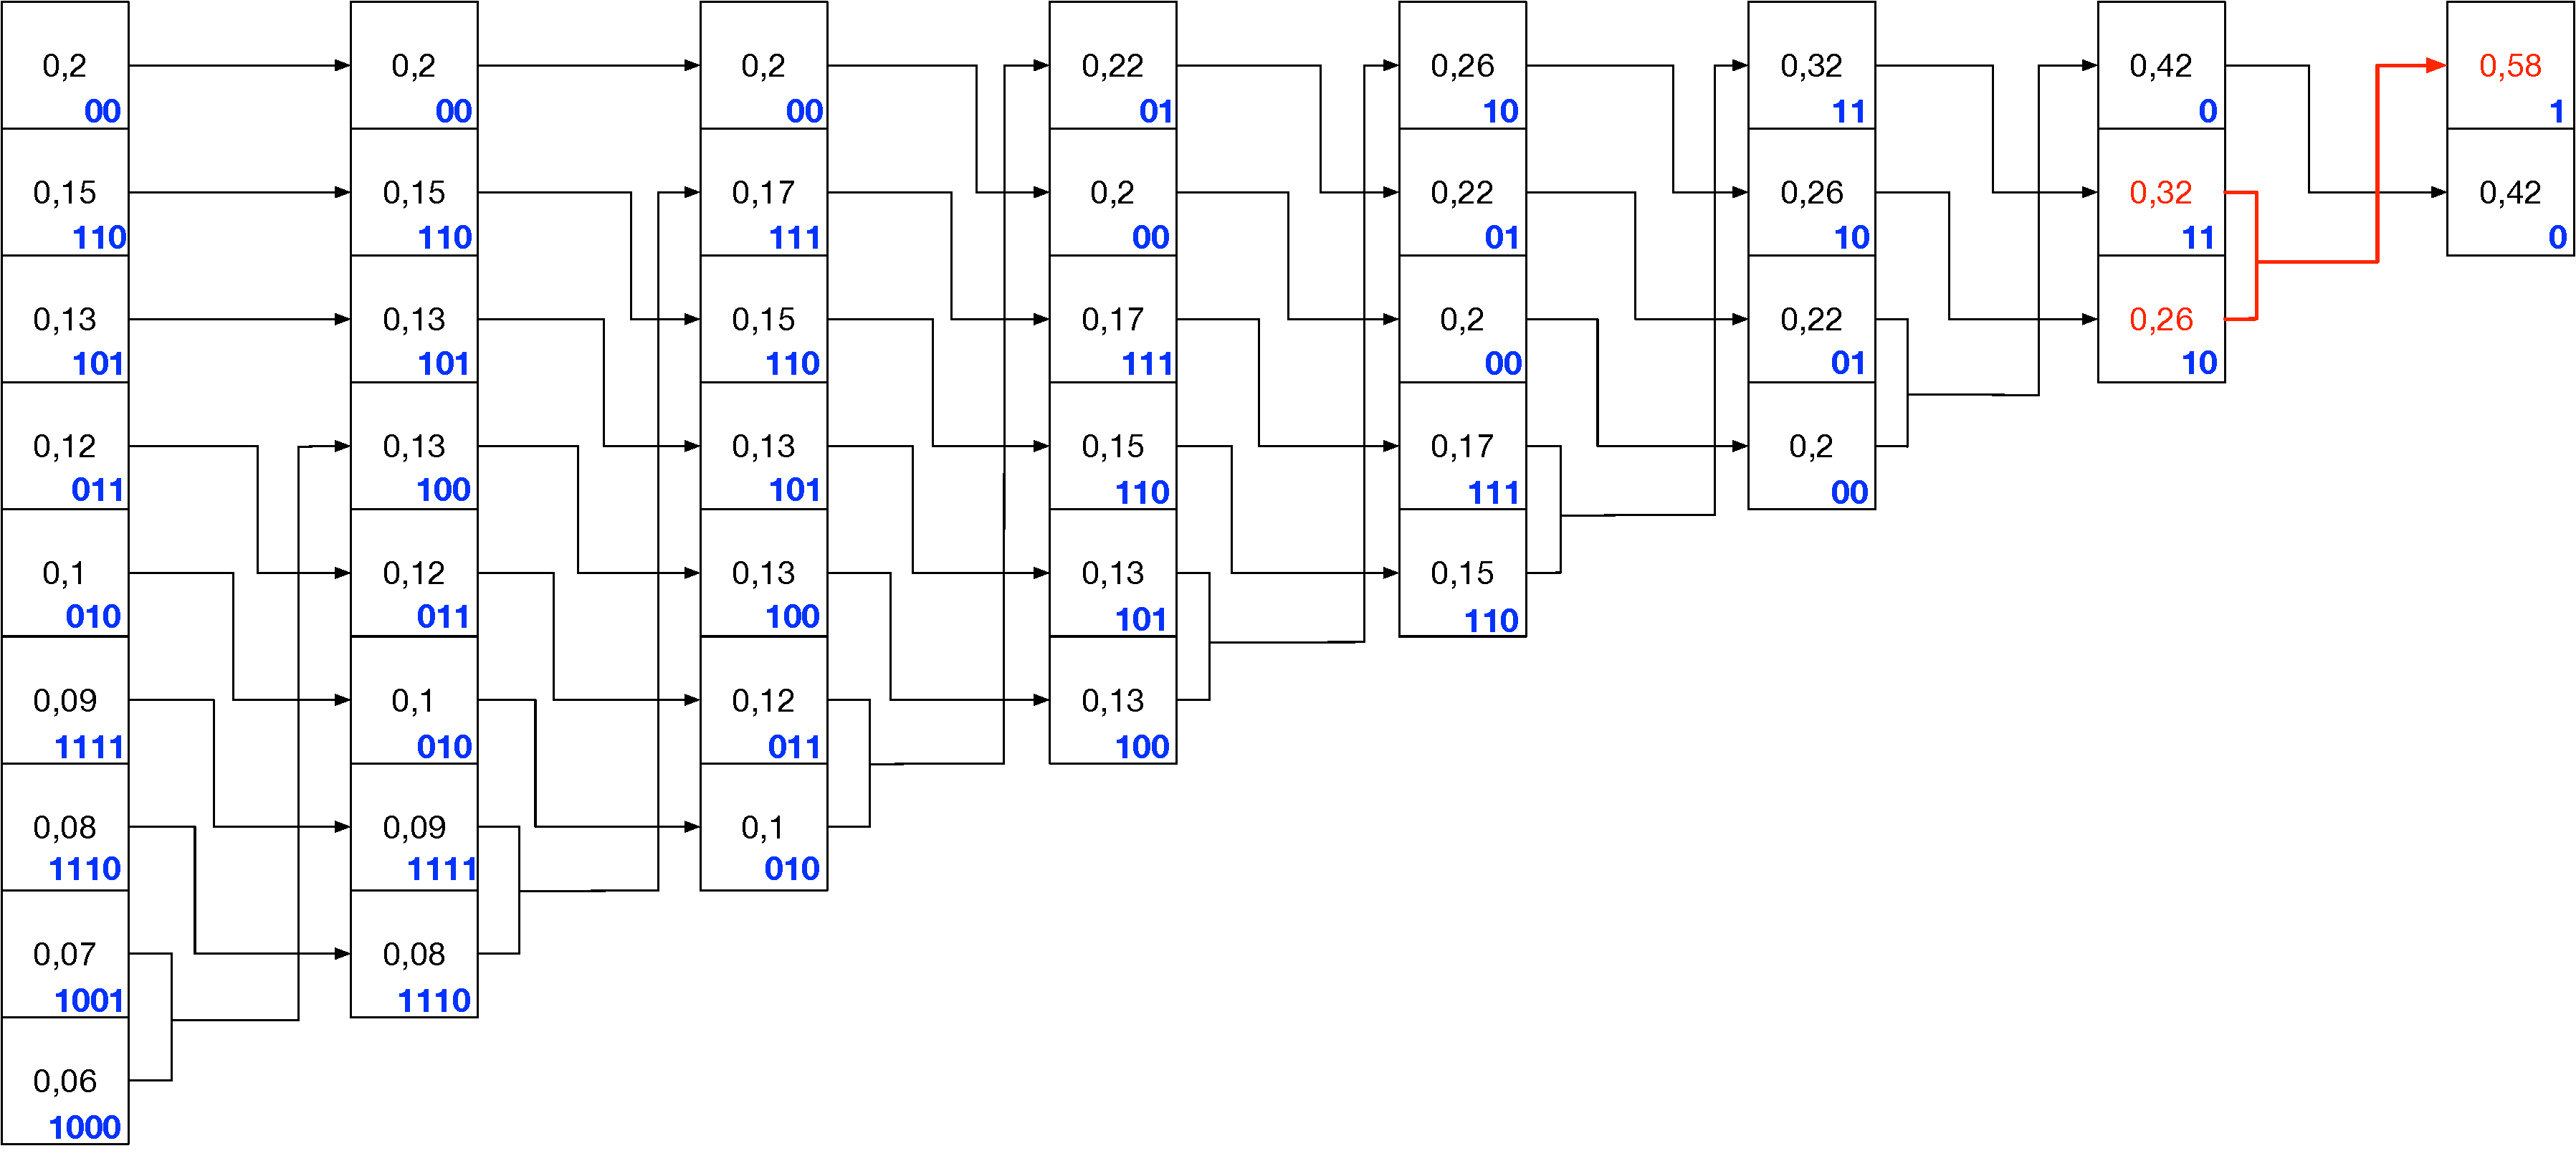
\includegraphics[height=5cm]{./Figuras/Huffman10.pdf}
\end{frame}

\begin{frame}{Codificación Huffman}{Ejemplo}
  \begin{itemize}
    \item Así, finalmente:
  \end{itemize}

  \begin{tabular}{|c|c|}
    \hline
    $0,2$ & $00$ \\
    \hline
    $0,15$ & $110$ \\
    \hline
    $0,13$ & $101$ \\
    \hline
    $0,12$ & $011$ \\
    \hline
    $0,1$ & $010$ \\
    \hline
    $0,09$ & $1111$ \\
    \hline
    $0,08$ & $1110$ \\
    \hline
    $0,07$ & $1001$ \\
    \hline
    $0,06$ & $1000$ \\
    \hline
  \end{tabular}
\end{frame}

\begin{frame}{Codificación Huffman}{Ejemplo}
  \begin{itemize}
    \item Longitud media:
    \begin{displaymath}
      \bar{L} = 2\cdot 0.2 + 3 \cdot (0.15 + 0.13 + 0.12 + 0.1) + 4 \cdot (0.09 + 0.08 + 0.07 + 0.06) = 3.1
    \end{displaymath}
    \item Se puede demostrar que se cumple que:
    \begin{displaymath}
      H \leq \bar{L} \leq H+1
    \end{displaymath}
  \end{itemize}

\end{frame}

\section{Codificación LZW}

\subsection{Definición}
\begin{frame}{Codificación LZW}{Definición}
	\begin{itemize}
    \item Tienen la ventaja de que no necesitamos conocer las probabilidades a priori de los símbolos.
    \item Se utiliza, por ejemplo, en los formatos de imagen GIF y TIFF.
	\end{itemize}
\end{frame}

\subsection{Pseudocódigo}
\begin{frame}[fragile]{Codificación LZW}{Pseudocódigo}
  \footnotesize
  \begin{verbatim}
    CADENA = cadena vacía
    WHILE queden caracteres por codificar DO
         CARACTER = coger el siguiente carácter
         IF CADENA+CARACTER está en el diccionario
              CADENA = CADENA+CARACTER
         ELSE
              código correspondiente a CADENA -> SALIDA
              Añadir CADENA+CARACTER al diccionario
              CADENA = CARACTER
         END
    END
     código para CADENA -> SALIDA
  \end{verbatim}
\end{frame}

\subsection{Ejemplo}
\begin{frame}{Codificación LZW}{Ejemplo}
	\begin{itemize}
    \item Supongamos que partimos del siguiente diccionario:

    \begin{tabular}{cc}
      Entrada & Código \\
      \hline
      a & 0 \\
      b & 1 \\
      n & 2 \\
    \end{tabular}
    \item El mensaje de entrada al codificador es: ``banana''
	\end{itemize}
\end{frame}

\begin{frame}{Codificación LZW}{Ejemplo}
	\begin{itemize}
    \item Siguiendo el proceso del pseudocódigo, vamos construyendo el diccionario y codificando el mensaje:
    \begin{tabular}{lcclc}
      CADENA & CARACTER  & ¿En el Diccionario? & Al Diccionario & Salida \\
      \hline
         & b & Si &  &  \\
       b & a & No & 3 - ba & 1 \\
       a & n & No & 4 - an & 0 \\
       n & a & No & 5 - na & 2 \\
       a & n & Sí & 		&  \\
       an & a & No & 6 - ana & 4 \\
       a & & & & 0 \\ 	
      \end{tabular}
    \item Al final, el mensaje codificado es: \texttt{1 0 2 4 0}.
	\end{itemize}
\end{frame}


\subsection{Decodificación}
\begin{frame}[fragile]{Codificación LZW}{Decodificación}
  \footnotesize
  \begin{verbatim}
    CODIGO_1 = Leer primer código del mensaje
    Traducción de CODIGO_1 -> SALIDA
    WHILE queden caracteres por decodificar
         CODIGO_2 = Leer siguiente código
         CADENA = traducción de CODIGO_2
         CADENA -> SALIDA
         CARACTER = Primer carácter de CADENA
         Añadir (Traducción de CODIGO_1)+(CARACTER) al diccionario
         CODIGO_1 = CODIGO_2
    END
\end{verbatim}
\end{frame}

\subsection{Ejemplo}
\begin{frame}{Codificación LZW}{Ejemplo}
	\begin{itemize}
    \item Siguiendo el proceso del pseudocódigo, vamos reconstruyendo el diccionario y decodificando el mensaje:
    \begin{tabular}{lccccc}
      CODIGO1 & CODIGO2  & CADENA & CARACTER & Salida & Dicc.\\
      \hline
      1 &   &   &   & b &\\
      1 & 0 & a & a & a & 3 - ba \\
      0 & 2 & n & n & n & 4 - an \\
      2 & 4 & an & a & an & 5 - na \\
      4 & 0 & a & a & a & 6 - ana \\
      \end{tabular}
	\end{itemize}
\end{frame}


\end{document}
